\documentclass{article}

\usepackage{amsmath} % Define various maths environments
\usepackage{amssymb} % Define various maths symbols
\usepackage{geometry} % Adjust the margin, paper size, and etc.
\geometry{a4paper, scale = 0.8}
\usepackage{enumerate} % Provide different style of lists
\usepackage{graphicx} % Insert image of all types
\usepackage{xcolor}
\usepackage{ulem}
\usepackage{pdfpages}
\usepackage{array} % Provide auxiliary farmat for tabular
\usepackage{booktabs} % Create Three-line Table
\usepackage{bm}
\usepackage{cite}
\usepackage{url}
\usepackage{float}
\usepackage{indentfirst}
\usepackage{multirow}
\usepackage[colorlinks,linkcolor=black]{hyperref}
\usepackage{subfigure}

\begin{document}

\vspace*{0.4cm}

\hrulefill %??????draw a horizontal line??????

\thispagestyle{empty} %set empty in footnote

\begin{center}
\begin{large}
\scshape{UM--SJTU Joint Institute \vspace{0.3em} \\ Physics Laboratory \\(Vp241)}
\end{large}

\hrulefill %??????draw a horizontal line??????

\vspace*{7.5cm}
\begin{Large}
\scshape{{Laboratory Report}}
\end{Large}

\vspace{2.5em}

\begin{large}
\scshape{Exercise 5}\\
\vspace{0.5em}
\scshape{RC, RL and RLC Circuit}
\end{large}
\end{center}

\vspace{13em}

\begin{table}[h!]
\center
\begin{tabular}{lll}
\textbf{Name: Haoming  Zhu} \hspace*{2em}&
\textbf{ID: 520021910145}\hspace*{2em}
& Group: 1 \\ \bottomrule
\end{tabular}
\end{table}

\vspace{-0.4cm}

\begin{center}
\hspace{0.3em} Date: 2021.12.3
\end{center}

\newpage
\tableofcontents
\setcounter{page}{0}
\thispagestyle{empty}
\newpage



		\section{Introduction}
	\subsection{Objective}
The objective of this lab is to study the properties of RC, RL, and RLC circuits. The charging and discharging process of each circuit is particularly studied. Also, the resonance phenomenon of RLC circuit is explored by studying the resonance frequency and quality factor.
	\subsection{RC Series Circuit}	
An $RC$ circuit consists of a capacitor, a resistor and a current source. For the charging process applying Kirchhoff’s loop rule, we get
\begin{equation}\label{RCloop}
RC\frac{dU_C}{dt}+U_C=\mathcal{E}
\end{equation}
solve the equation, the voltage across the capacitor is then
$$U_C = \mathcal{E}(1-e^{-\frac{t}{RC}})~~\text{and}~~U_R = iR = \mathcal{E}e^{-\frac{t}{RC}}$$

For the discharging process, we just need to replace the $rhs$ of Eq. \eqref{RCloop} with 0, then we can get $$U_C = U_R = \mathcal{E}e^{-\frac{t}{RC}}$$

The $\textit{time constant}$ of the circuit is defined to be $\tau = RC$. The half-life period is defined to be the time needed for $U_C$ to decrease to half of the initial value or increase to half of the terminal value. By their definition and the expression of $U_C$, it can be derived that

\begin{equation}
    T_{1/2} = \tau\ln 2.
    \label{eq:ThalfRC}
\end{equation}


\begin{figure}[H]
\centering
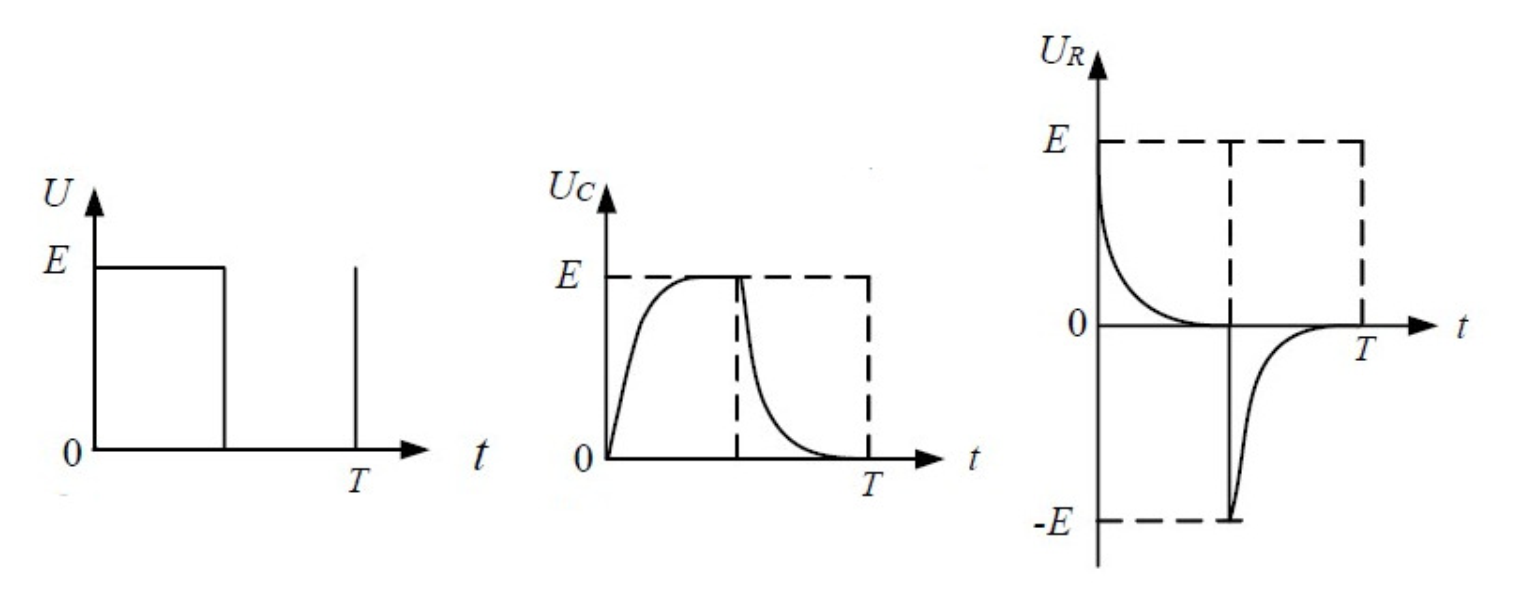
\includegraphics[scale=0.5]{RC}
\caption{Charging/discharging curves for a $RC$ series circuit.}
\end{figure}

\subsubsection{$RL$ Series Circuit}
An $RL$ consists of an inductor and a resistance. Similarly, the time constant $\tau = \frac{L}{R}$
and still
\begin{equation}
    T_{1/2} = \tau\ln 2.
    \label{eq:ThalfRL}
\end{equation}

	\subsubsection{RLC Series Circuit}
An $RLC$ circuit consists of an inductor, a capacitor and a resistor. By KVL, we can obtain a second order ordinary differential equation	 $w.r.t.$ the voltage in the loop:
\begin{equation}
  LC\frac{\mathrm{d}^2U_C}{\mathrm{d}t^2} + RC\frac{\mathrm{d}U_C}{\mathrm{d}t} + U_C = \mathcal{E},
\end{equation}

Dividing both sides of the equation by $LC$ and introducing the symbols
$$    \beta = \frac{R}{2L},\hspace{2em} \text{and} \hspace{2em}\omega_0 = \frac{1}{\sqrt{LC}},$$
it can be rewritten as
\begin{equation}
  \frac{\mathrm{d}^2U_C}{\mathrm{d}t^2} + 2\beta\frac{\mathrm{d}U_C}{\mathrm{d}t} + \omega_0^2U_C = \omega_0^2\mathcal{E},
\end{equation}
with initial conditions
$$U_C(t=0) = 0\hspace{2em} \text{and} \hspace{2em}\frac{\mathrm{d}U_C}{\mathrm{d}t}\bigg|_{t=0} = 0.$$

Given different values of $\beta$ and $\omega_0$, there are three regimes, as implied by the solution of the complementary homogeneous equation: 

$\blacktriangleright$ If $\beta^2 - \omega_0^2 < 0$ (weak damping), the system is in the underdamped regime and the solution to the initial value problem is of the form
$$U_C = \mathcal{E} - \mathcal{E}e^{-\beta t}(\cos\omega t +\frac{\beta}{\omega}\sin \omega t),$$
where $\omega = \sqrt{\omega_0^2 - \beta^2}$.

$\blacktriangleright$ If $\beta^2 - \omega_0^2 > 0$ (strong damping), the system is in the overdamped regime with the solution of the form
$$U_C = \mathcal{E} - \frac{\mathcal{E}}{2\gamma}e^{-\beta t}[(\beta + \gamma)e^{\gamma t} - (\beta -\gamma)e^{-\gamma t}],$$
where $\gamma = \sqrt{\beta^2 - \omega_0^2}$.

$\blacktriangleright$ Finally, if $\beta^2 - \omega_0^2 = 0$, the system is said to be critically damped, and

$$U_C = \mathcal{E} - \mathcal{E}(1+\beta t)e^{-\beta t}.$$

When the $RLC$ circuit system is \textbf{critically damped}, the time constant and can be obtained using $T_{0.264}$ through
\begin{equation}
    \tau = \frac{T_{0.264}}{1.00} = \sqrt{LC}.
    \label{eq:ThalfRLC}
\end{equation}

The three regimes are shown below.
\begin{figure}[H]
\centering
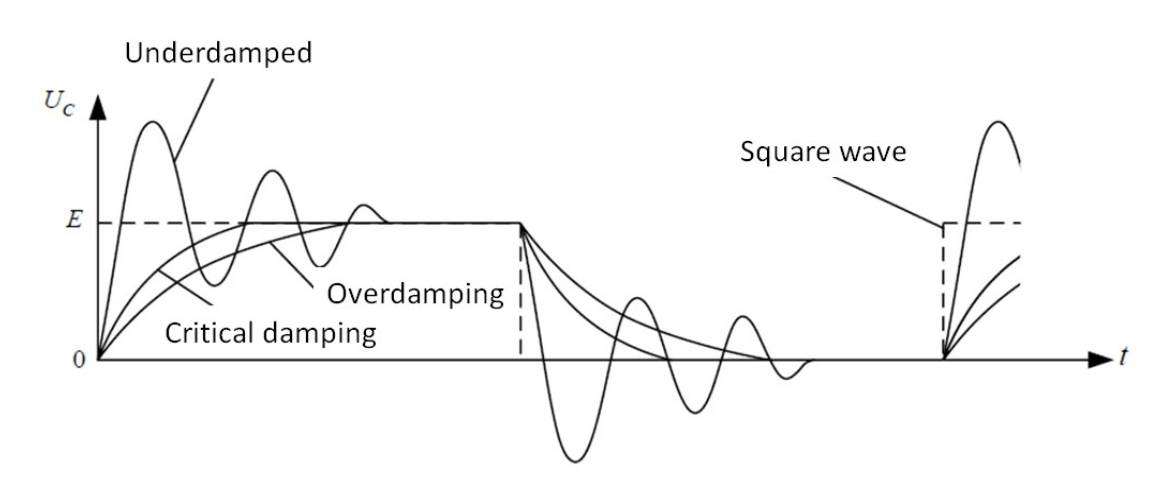
\includegraphics[scale=0.5]{3damp}
\caption{Three different regimes of transient processes in a $RLC$ series circuit.}
\end{figure}

\subsection{$RLC$ Resonant Circuit}

\subsubsection{Phase Shift and Resonance Frequency}
We know that in AC circuit
$$
Z_R = R\hspace{2em}Z_C = \frac{j}{\omega C}\hspace{2em}Z_L = j\omega L
$$
Then according to the rule of complex magnitude, the total impedance is
\begin{equation*}\label{EqZ}
    Z = \sqrt{R^2 + \bigg(\omega L - \frac{1}{\omega C}\bigg)^2},
\end{equation*}
with the phase difference between the current and the voltage in the circuit

\begin{equation}
    \varphi = \tan^{-1}\bigg(\frac{\omega L - \frac{1}{\omega C}}{R}\bigg).
    \label{eq:phitheo}
\end{equation}

\subsubsection{Resonance}

If the frequency of the input signal provided by the source satisfies
$$\omega_0 L = \frac{1}{\omega_0 C}, \hspace{2em} \text{which gives} \hspace{2em} \omega_0 = \frac{1}{\sqrt{LC}},$$
the total impedance will reach a minimum, $Z_0 = R$. Correspondingly, the current reaches its maximum, $I_m = U/R$. Then the circuit is said to be at resonance. The theoretical resonance frequency is then 
\begin{equation}
    f_0 = \frac{\omega_0}{2\pi} = \frac{1}{2\pi\sqrt{LC}},
    \label{eq:fres}
\end{equation}

\subsubsection{Quality Factor in Resonant Circuits}

For a circuit driven at the resonance frequency, the ratio of $U_L$ (or $U_C$) to $U$ is called the quality factor $Q$ of a resonant circuits

\begin{equation}
    Q = \frac{U_L}{U} = \frac{\omega_0 L}{R} \hspace{2em} \text{or} \hspace{2em} Q = \frac{U_C}{U} = \frac{1}{\omega_0 RC} =  \frac{\sqrt{LC}}{RC}.
    \label{eq:Qtheo}
\end{equation}

The quality factor is then

\begin{equation}
    Q = \frac{f_0}{f_2 - f_1},
    \label{eq:Qex}
\end{equation}
where $f_1$ and $f_2$ are two frequencies such that $I(f_1) = I(f_2) = I_\text{m}/\sqrt{2}$.



\section{Apparatus}

The measurement devices consists of a signal generator, an oscilloscope, a digital multimeter, a wiring board, a fixed resistor 100 $\Omega$ (2 W), a variable resistor 2 $\text{k}\Omega$ (2 W), two capacitors 0.47 $\mu \text{F}$ and 0.1 $\mu\text{F}$, and two inductors (10 mH and 33 mH).

The precisions of the apparatus are shown below. The 10 mH inductor used in this lab is precise, and we consider it as 0 uncertainty.

\begin{table}[H]
    \centering
    \begin{tabular}{ccc}
        \toprule
        Apparatus                           & Quantity measured & Uncertainty               \\
        \midrule
        \multirow{2}{*}{Signal generator}   & Frequency         & 0.001 Hz                          \\
                                            & Amplitude         & 0.001 $\text{V}_{\text{pp}}$      \\ \hline
        \multirow{2}{*}{Oscilloscope}       & Time & 0.01/0.001 $\mu\text{s}$          \\
                                            & Voltage           & 0.02/0.002 $\text{V}_{\text{pp}}$ \\ \hline
        \multirow{2}{*}{Digital multimeter} & Resistance        & 0.01 $\Omega$                     \\
                                            & Capacitance       & 0.01 nF                       \\
        \bottomrule
    \end{tabular}
    \caption{Precision of the measurement instruments.}\label{tablePresicion}
\end{table}

\newpage

\section{Measurement Procedure}

\subsection{$RC$, $RL$ Series Circuit}
In this part, the wave forms of $RC$ and $RL$ circuits are studied.

First, I chose a capacitor labelled with 0.1 $\mu F$ and a inductor labelled with 10 $mF$ to connect with a resistor labelled with 100 $\Omega$ to form two circuits respectively. Note that in the $RC$ circuit, the voltage across the capacitor is measured through oscilloscope, while in the $RL$ circuit the voltage across the resistor is measured.

Next, I adjusted the oscilloscope and measured $T_{0.264}$ for the two circuits respectively. Then, the time constant can be calculated and compared with the theoretical value. Also, I took screen shots for the two wave forms.

\subsection{$RLC$ Series Circuit}

In this part, the wave forms of $RLC$ circuit under different regimes are studied, including under-damped, critically damped, and over-damped regimes.

First, I connected the $0.1\mu F$ capacitor, the 10 $mF$ inductor and a rheostat in series. Then, I adjusted the rheostat to obtain the three regimes and took three screen shots. 

Next, I adjusted the rheostat to to obtain critical damped again and find the corresponding parameters of $T_{0.264}$ to find the time constant.


\subsection{$RLC$ Resonant Circuit}

In this part, the $RLC$ circuit under resonance is studied to find the quality factor $Q$.

First, the power source's wave form is shifted to sinusoidal waves. Then, I adjusted the input frequency until the circuit reach the resonant state and recorded the frequency. Next, below and beyond the resonant frequency, I took another 20 frequencies that have same voltages in symmetry. Finally, I lotted the graphs $f/f_0$ vs. $I/I_\text{m}$ and $f/f_0$ vs. $\varphi$ to estimate the resonance frequency and calculate the quality factor $Q$.


\section{Results}

\subsection{$RC$ Series Circuit}

The measured data for the $RC$ series are shown in Table \ref{TableRC}.

\begin{table}[H]
    \centering
    \begin{tabular}{c|c}
        \toprule
        Quantity & Value \\
        \midrule
        $R\,\,[\Omega]$ & 99.75 $\pm$ 0.01 \\
        $f\,\,[\text{Hz}]$ & 1000.000 $\pm$ 0.001 \\
        $C$ [nF] & 99.84 $\pm$ 0.01 \\
        $\mathcal{E}\,\,[\text{V}_{\text{pp}}]$ & 4.000 $\pm$ 0.001    \\
        $T_{1/2}\,\,[\mu\text{s}]$  & 7.000 $\pm$ 0.001  \\
        \bottomrule
    \end{tabular}
    \caption{$T_{1/2}$ measurement data for a $RC$ series circuit.\label{TableRC}}
\end{table}

According to Eq.\eqref{eq:ThalfRC}, the experimental time constant $\tau$ can be calculated as
$$\tau = \frac{T_{1/2}}{\ln 2} = \frac{7.000}{\ln 2} = 10.0989\pm 0.0014 \,\,[\mu\text{s}].$$

According to the capacitor and resistor used in the circuit, the theoretical value $\tau_{theo}$ for this $RC$ circuit is
$$\tau_{\text{theo}} = RC = 99.75 \times 99.84 \times 10^{-3} = 9.96 \pm 0.10 \,\,[\mu\text{s}].$$

The relative deviation $u_r$ is then
$$u_r = \frac{|\tau-\tau_{\text{theo}}|}{\tau_{\text{theo}}} \times 100\% = \frac{10.0989-9.96}{9.9590} \times 100\% = 1.4\%.$$

Figure \ref{RCwave} shows the wave form of the $RC$ circuit.

\begin{figure}[H]
\centering
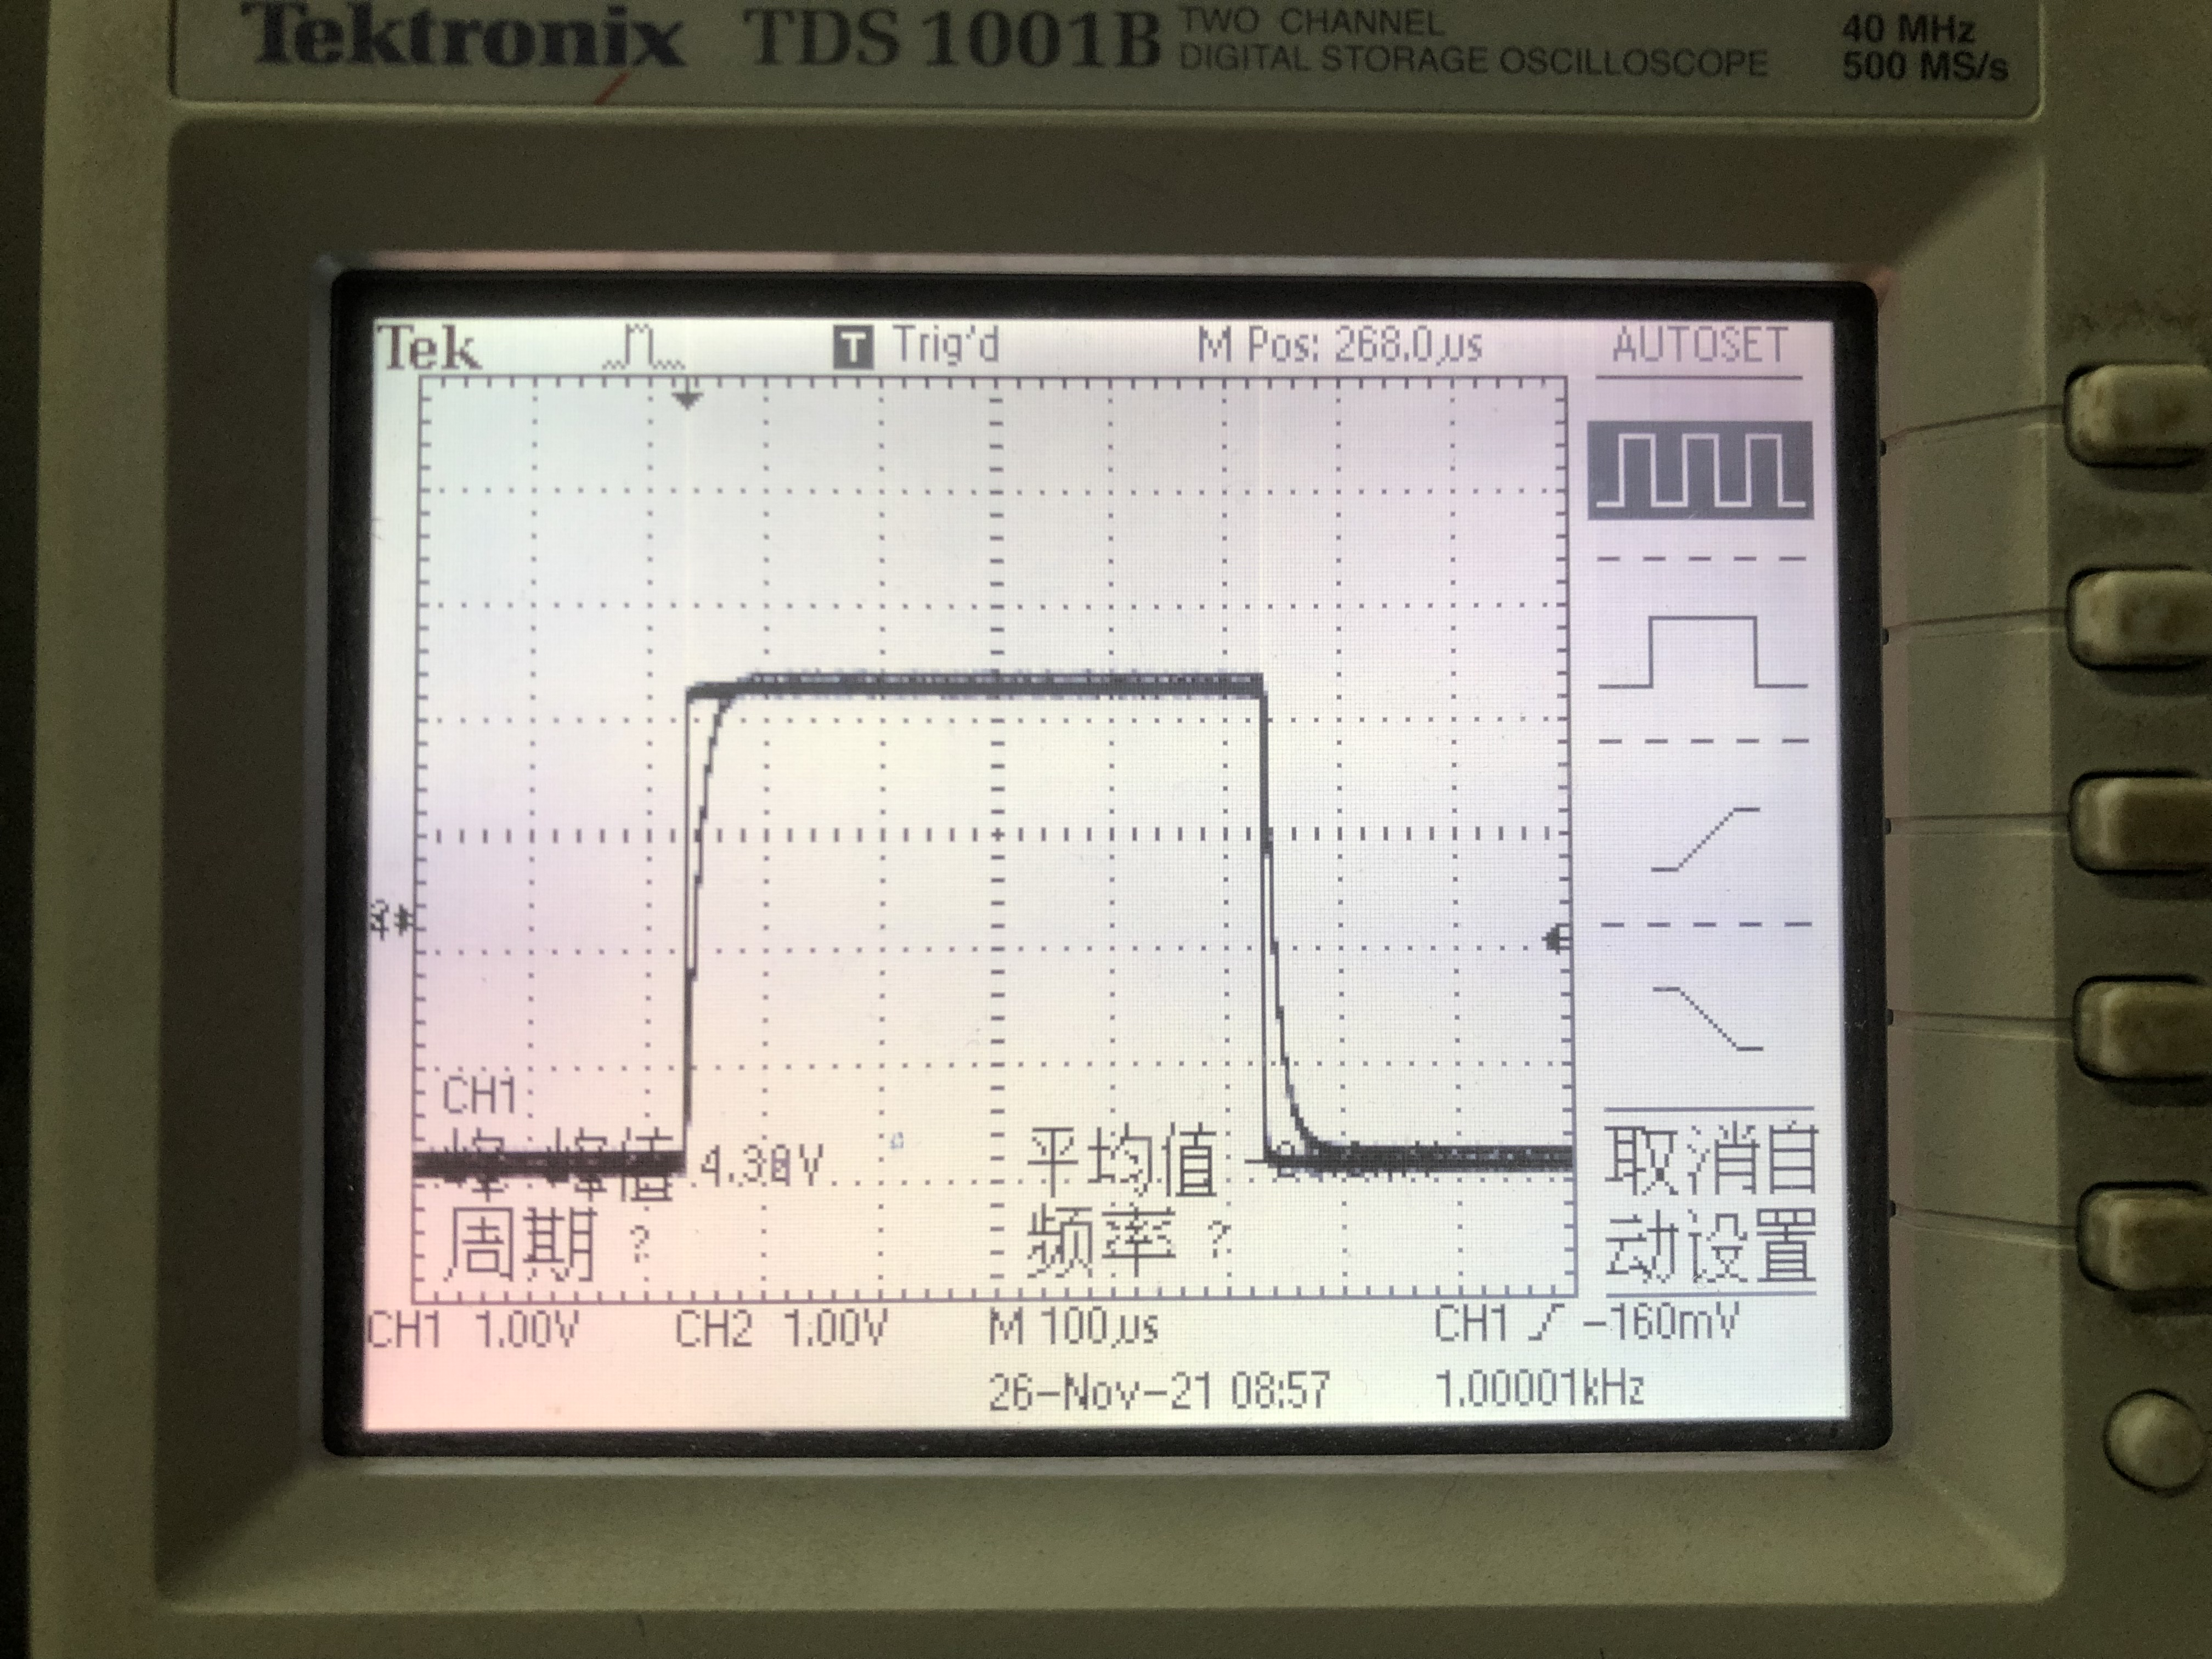
\includegraphics[scale=0.075]{RCwave.jpeg}
\caption{Wave form of a $RC$ series circuit.}\label{RCwave}
\end{figure}

\subsection{$RL$ Series Circuit}

The measured data for the $RL$ series are shown in Table \ref{TableRL}.

\begin{table}[H]
    \centering
    \begin{tabular}{c|c}
\toprule
        Quantity & Value \\
        \midrule
        $R\,\,[\Omega]$ & 99.75 $\pm$ 0.01 \\
        $f\,\,[\text{Hz}]$ & 1000.000 $\pm$ 0.001 \\
        $L$ [H] & 0.01 $\pm$ 0 \\
        $\mathcal{E}\,\,[\text{V}_{\text{pp}}]$ & 4.000 $\pm$ 0.001    \\
        $T_{1/2}\,\,[\mu\text{s}]$  & 66.00 $\pm$ 0.01  \\
        \bottomrule
    \end{tabular}
    \caption{$T_{1/2}$ measurement data for a $RL$ series circuit.\label{TableRL}}
\end{table}

According to the Eq.\eqref{eq:ThalfRL}, the experimental time constant $\tau$ can be calculated as
$$\tau = \frac{T_{1/2}}{\ln 2} = \frac{66.00}{\ln 2} = 95.218 \pm 0.014 \,\,[\mu\text{s}].$$

According to the inductor and resistor used in the circuit, the theoretical value $\tau_{theo}$ for this $RL$ circuit is
$$\tau_{\text{theo}} = \frac{L}{R} = \frac{0.01}{99.75} \times 10^{6} = 100.261 \pm 0.010 \,\,[\mu\text{s}].$$

The relative deviation $u_r$ is then
$$u_r = \frac{|\tau-\tau_{\text{theo}}|}{\tau_{\text{theo}}} \times 100\% = \frac{100.261 - 95.218}{100.261} \times 100\% = 5\%.$$

Figure \ref{RLwave} shows the wave form of the $RC$ circuit.

\begin{figure}[H]
\centering
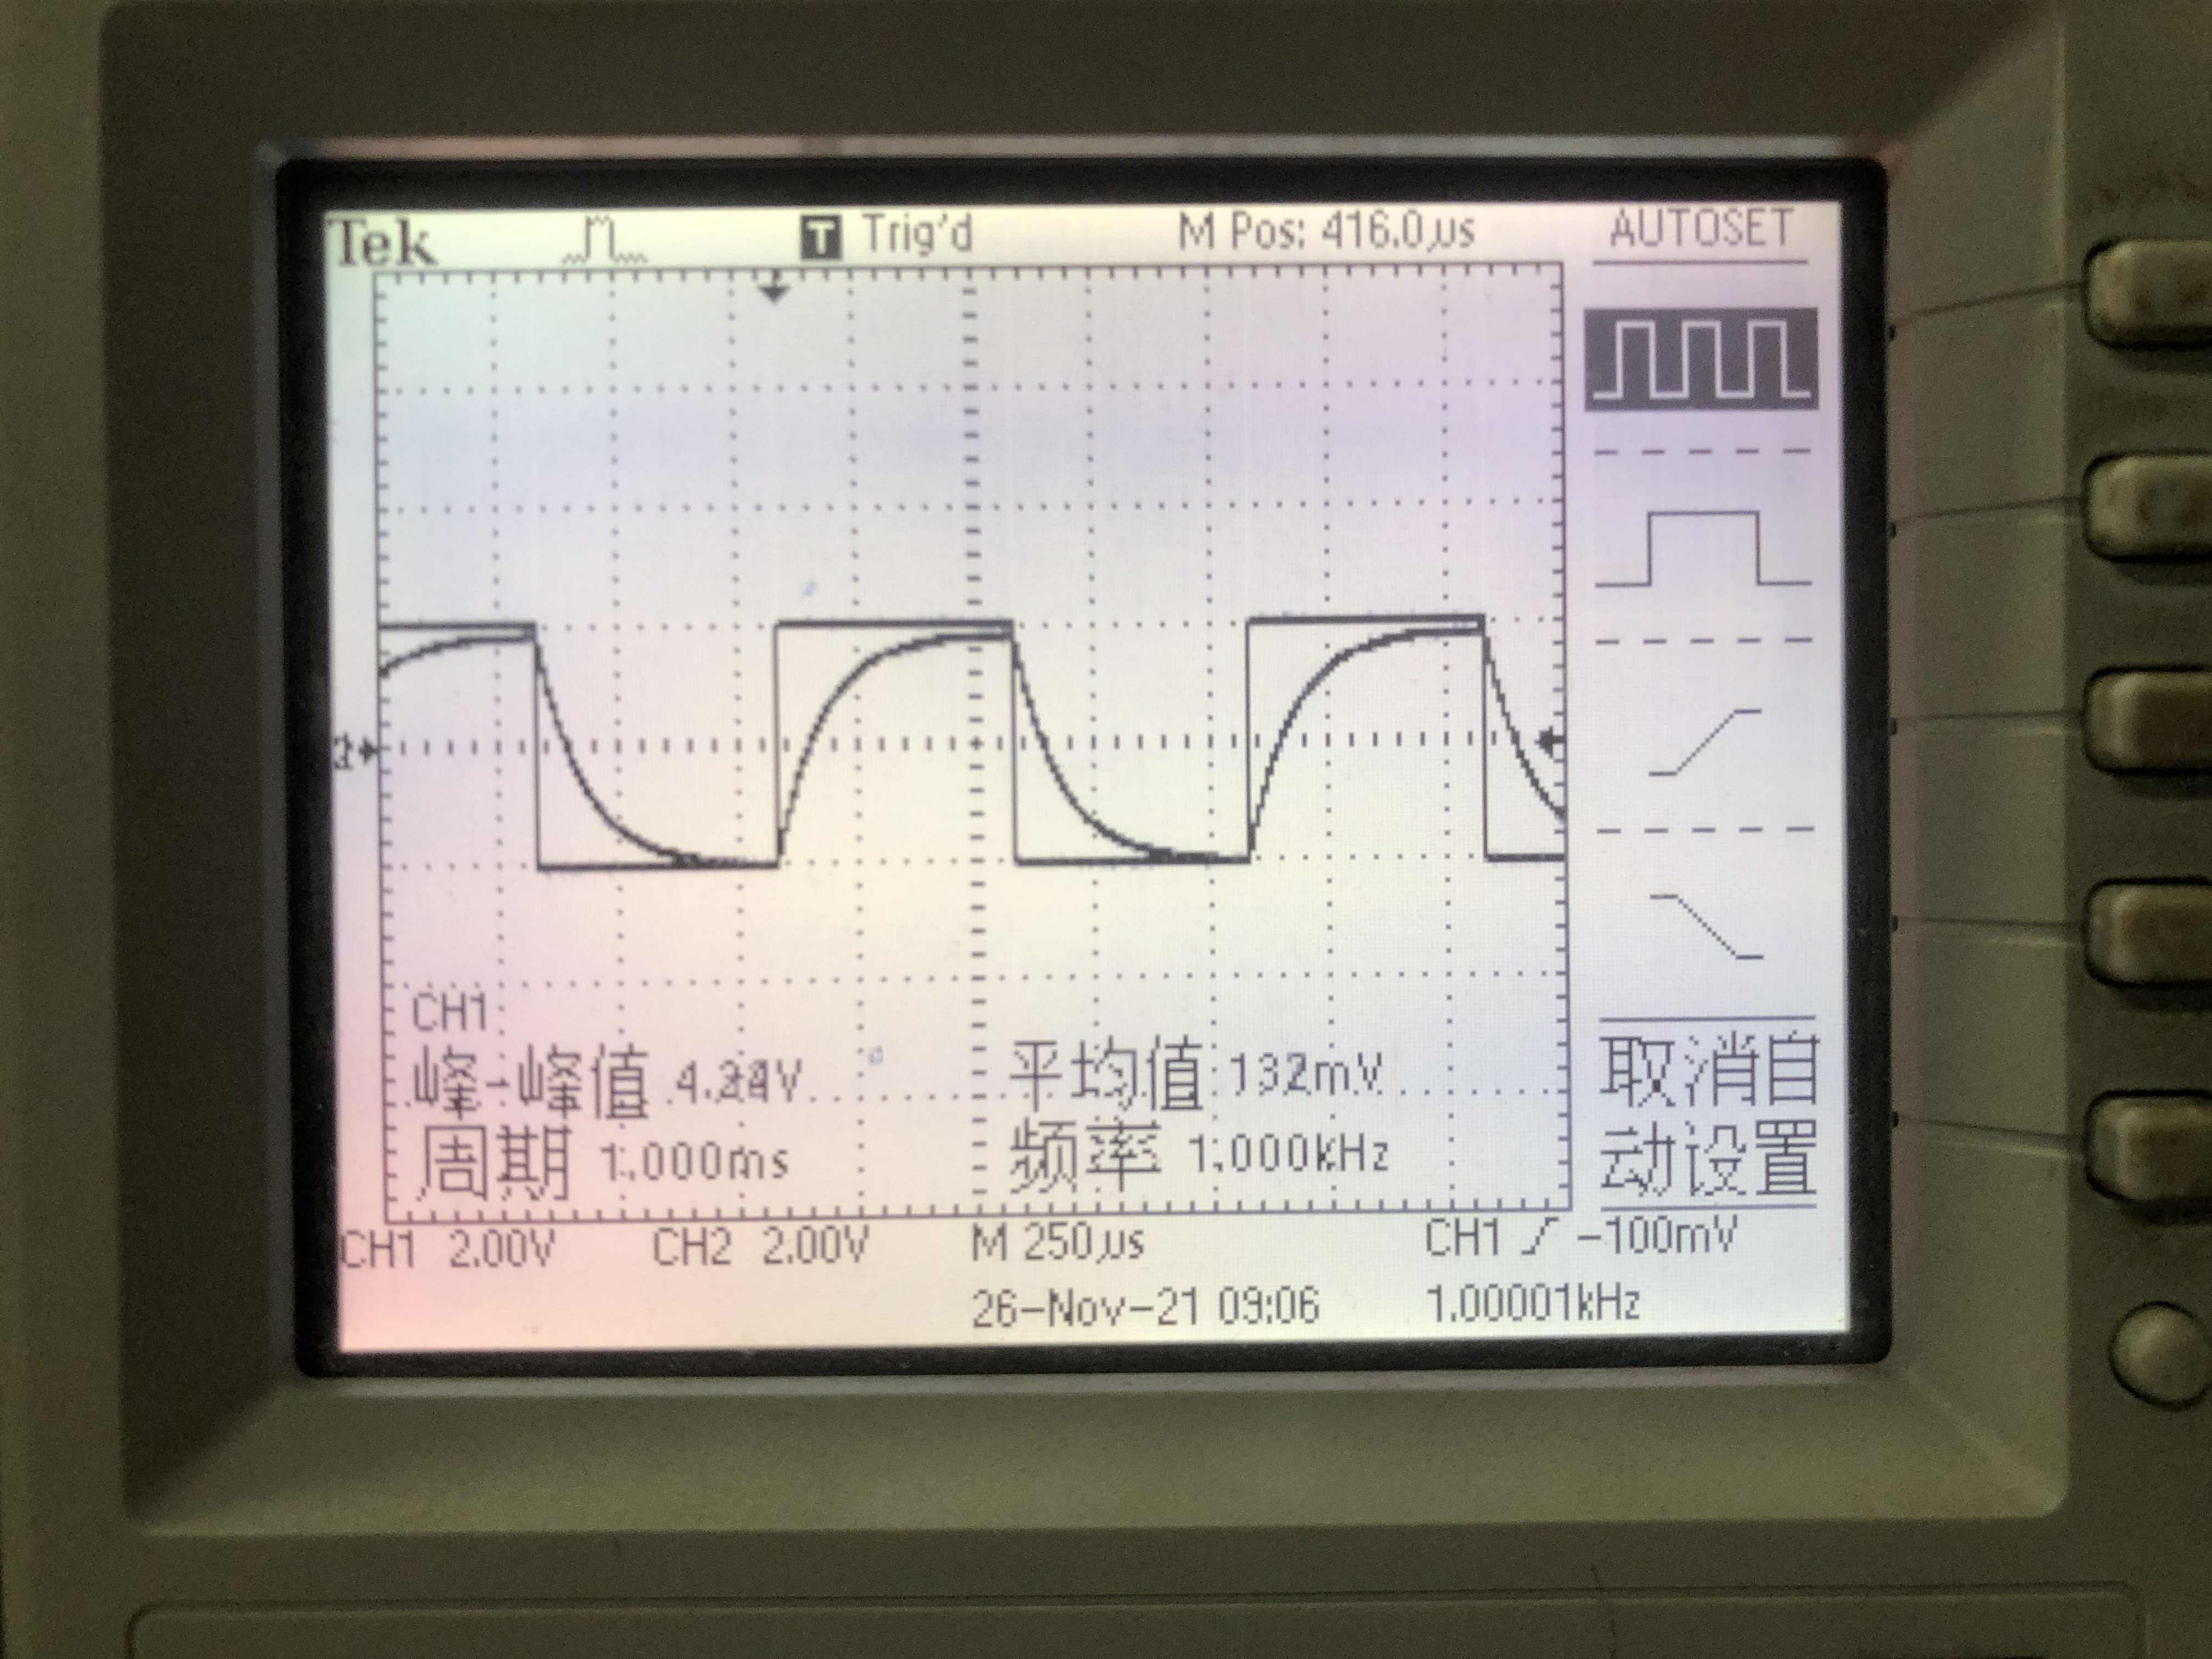
\includegraphics[scale=0.075]{RLwave.jpeg}
\caption{Wave form of a $RL$ series circuit.}\label{RLwave}
\end{figure}

\subsection{$RLC$ Series Circuit}

The measured data for the $RLC$ circuit are shown in Table \ref{TableRLC}.

\begin{table}[H]\centering
    \begin{tabular}{c|c}
    \toprule
            Quantity & Value \\
        \midrule
        $f\,\,[\text{Hz}]$ & 1000.000 $\pm$ 0.001 \\
        $C$ [nF] & 99.84 $\pm$ 0.01 \\
        $L$ [H] & 0.01 $\pm$ 0 \\
        $\mathcal{E}\,\,[\text{V}_{\text{pp}}]$ & 4.000 $\pm$ 0.001    \\
        $T_{0.264}\,\,[\mu\text{s}]$  & 30.00 $\pm$ 0.01  \\
        \bottomrule
    \end{tabular}
    \caption{$T_{1/2}$ measurement data for a critically damped $RLC$ series circuit.}\label{TableRLC}
\end{table}

Accordint to Eq.\eqref{eq:ThalfRLC}, the experimental time constant $\tau$ can be calculated as
$$\tau = T_{0.264} = 30.00 \pm 0.01\,\,[\mu\text{s}],$$

According to the elements used in the circuit, the theoretical value $\tau_{theo}$ for this $RLC$ circuit is
$$\tau_{\text{theo}} = \sqrt{LC} = \sqrt{0.01 \times 99.82 \times 10^{-9}} \times 10^{6} = 31.5975 \pm 0.0016 \,\,[\mu\text{s}].$$

The relative deviation $u_r$ is then
$$u_r = \frac{|\tau-\tau_{\text{theo}}|}{\tau_{\text{theo}}} \times 100\% = \frac{31.5943 - 30.00}{31.5943} \times 100\% = 5\%.$$


Figure \ref{RLCwave} shows the three wave forms of different regimes of the $RC$ circuit.

\begin{figure}[H]
\centering
\subfigure[Under-damped regime of the $RLC$ circuit.]{
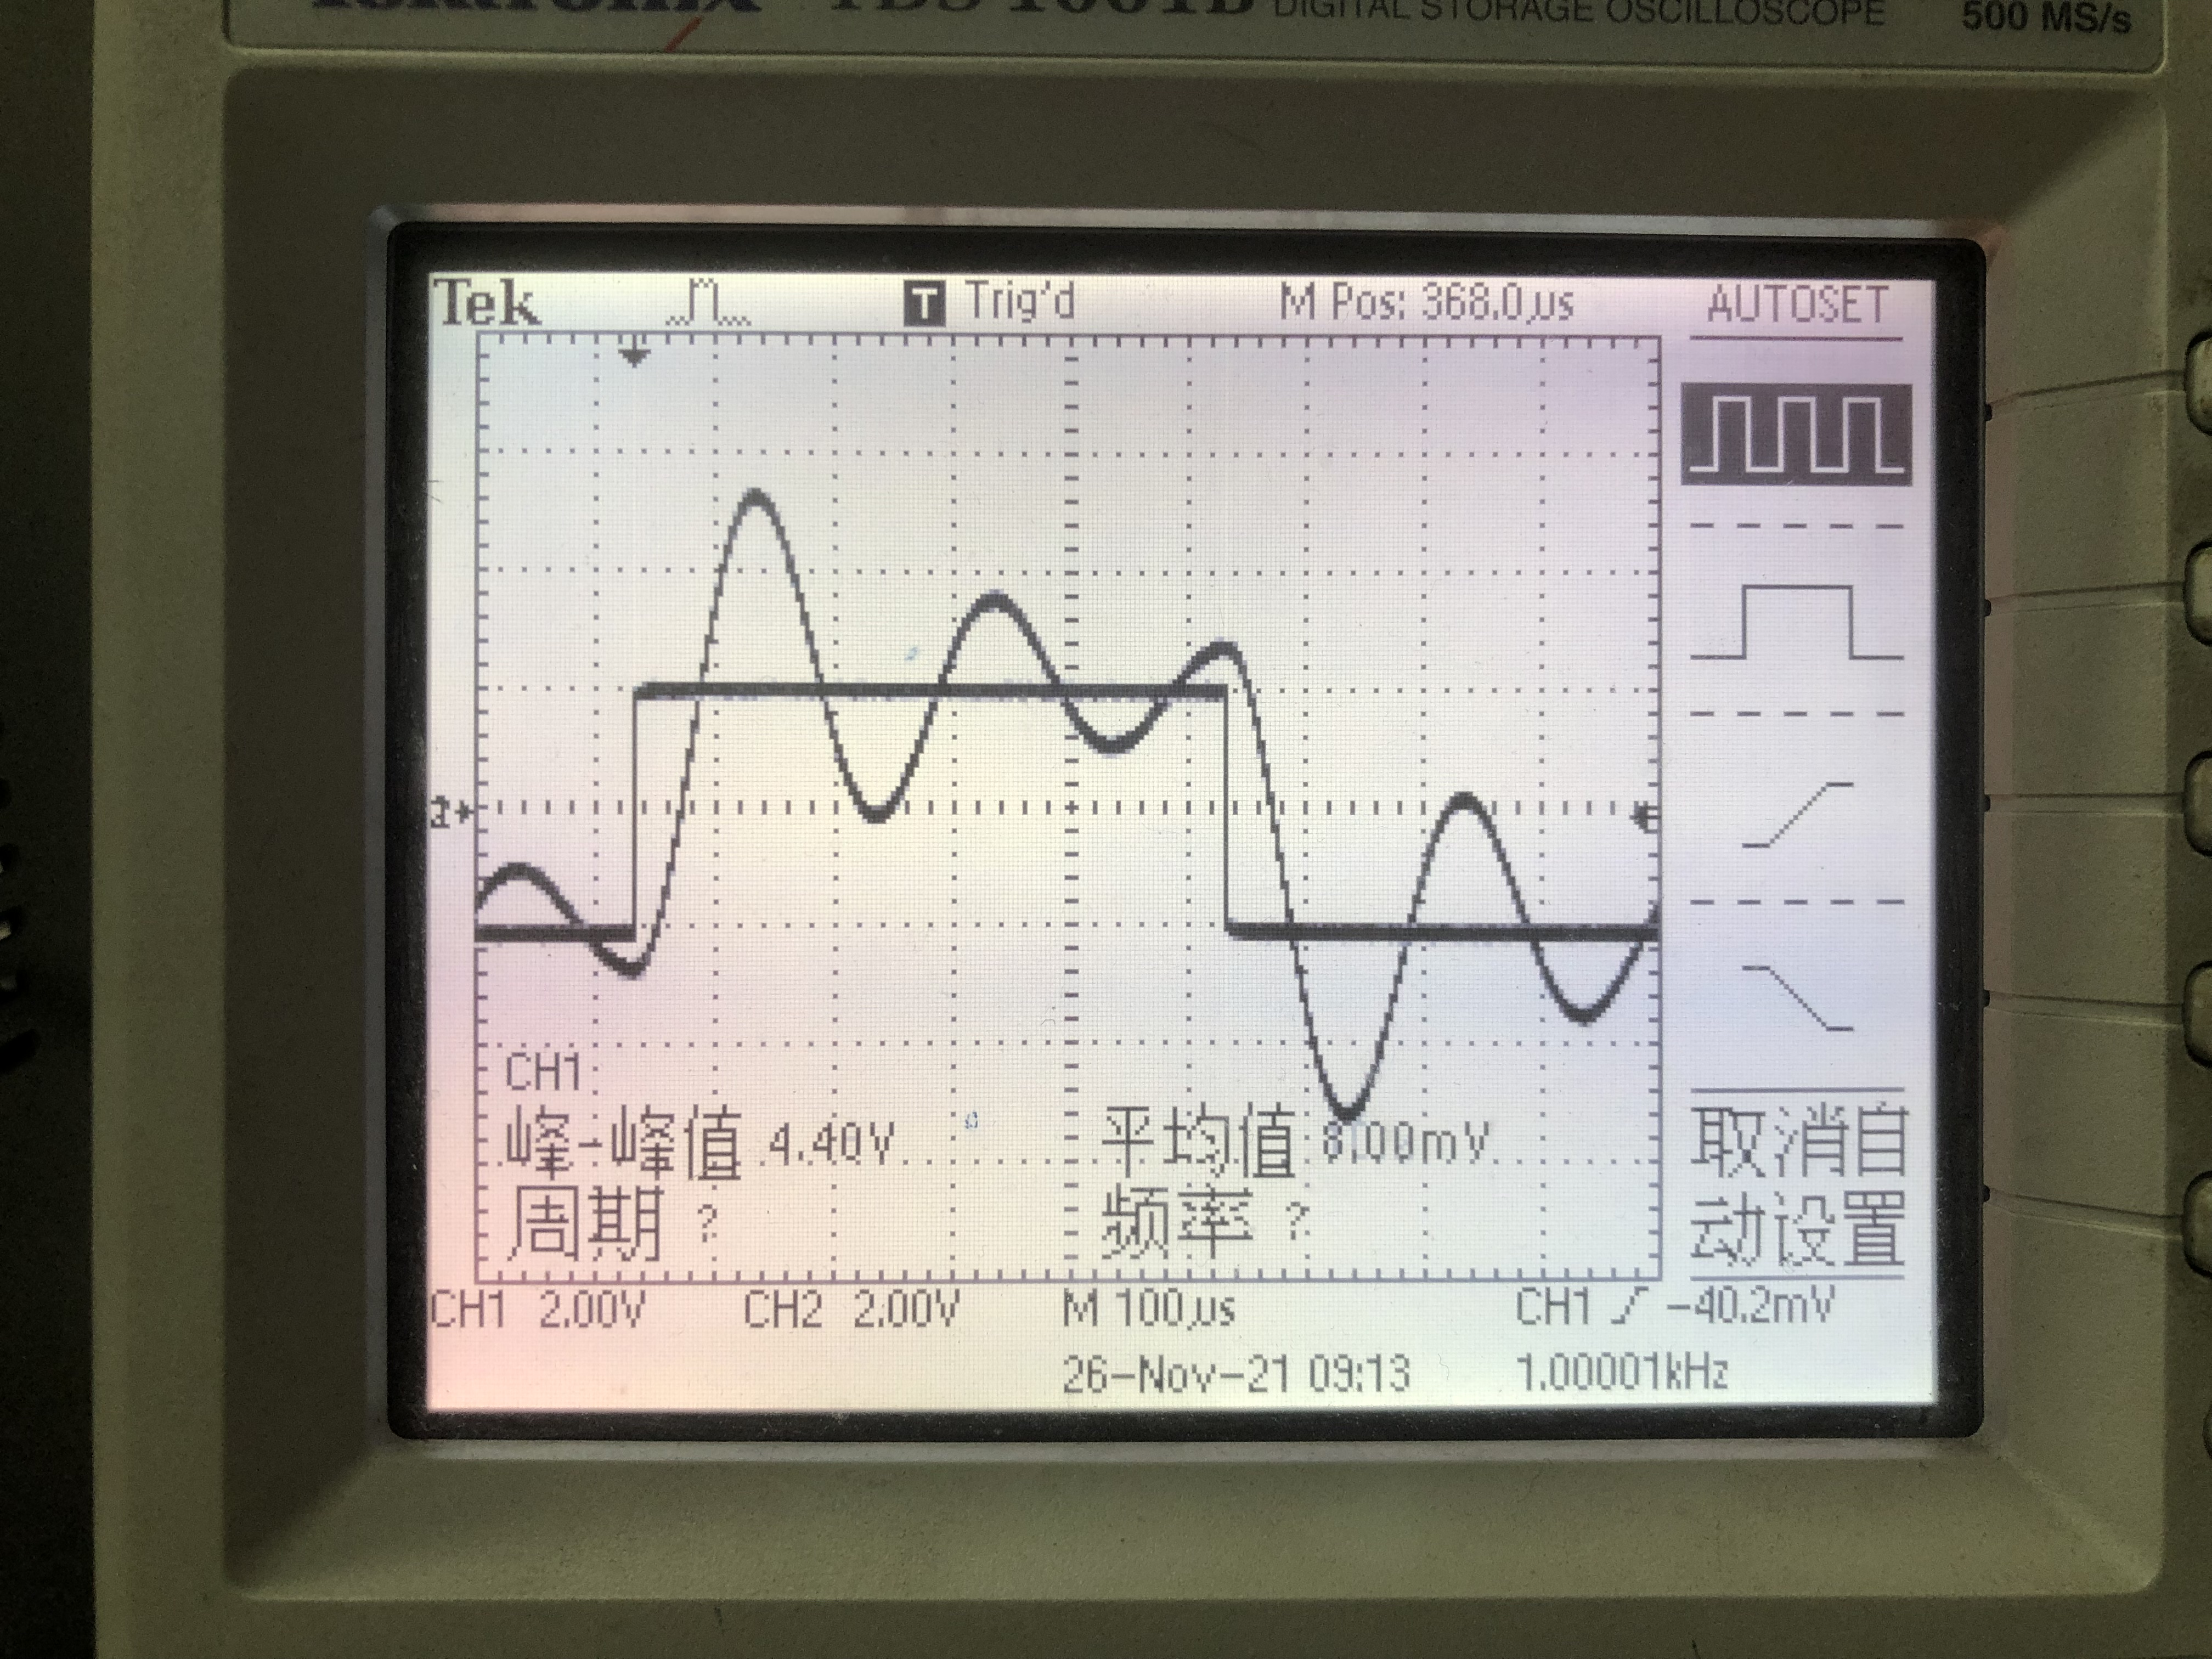
\includegraphics[width=3.5in]{under}\label{a}
}%

\subfigure[Critical-damped regime of the $RLC$ circuit.]{
\centering
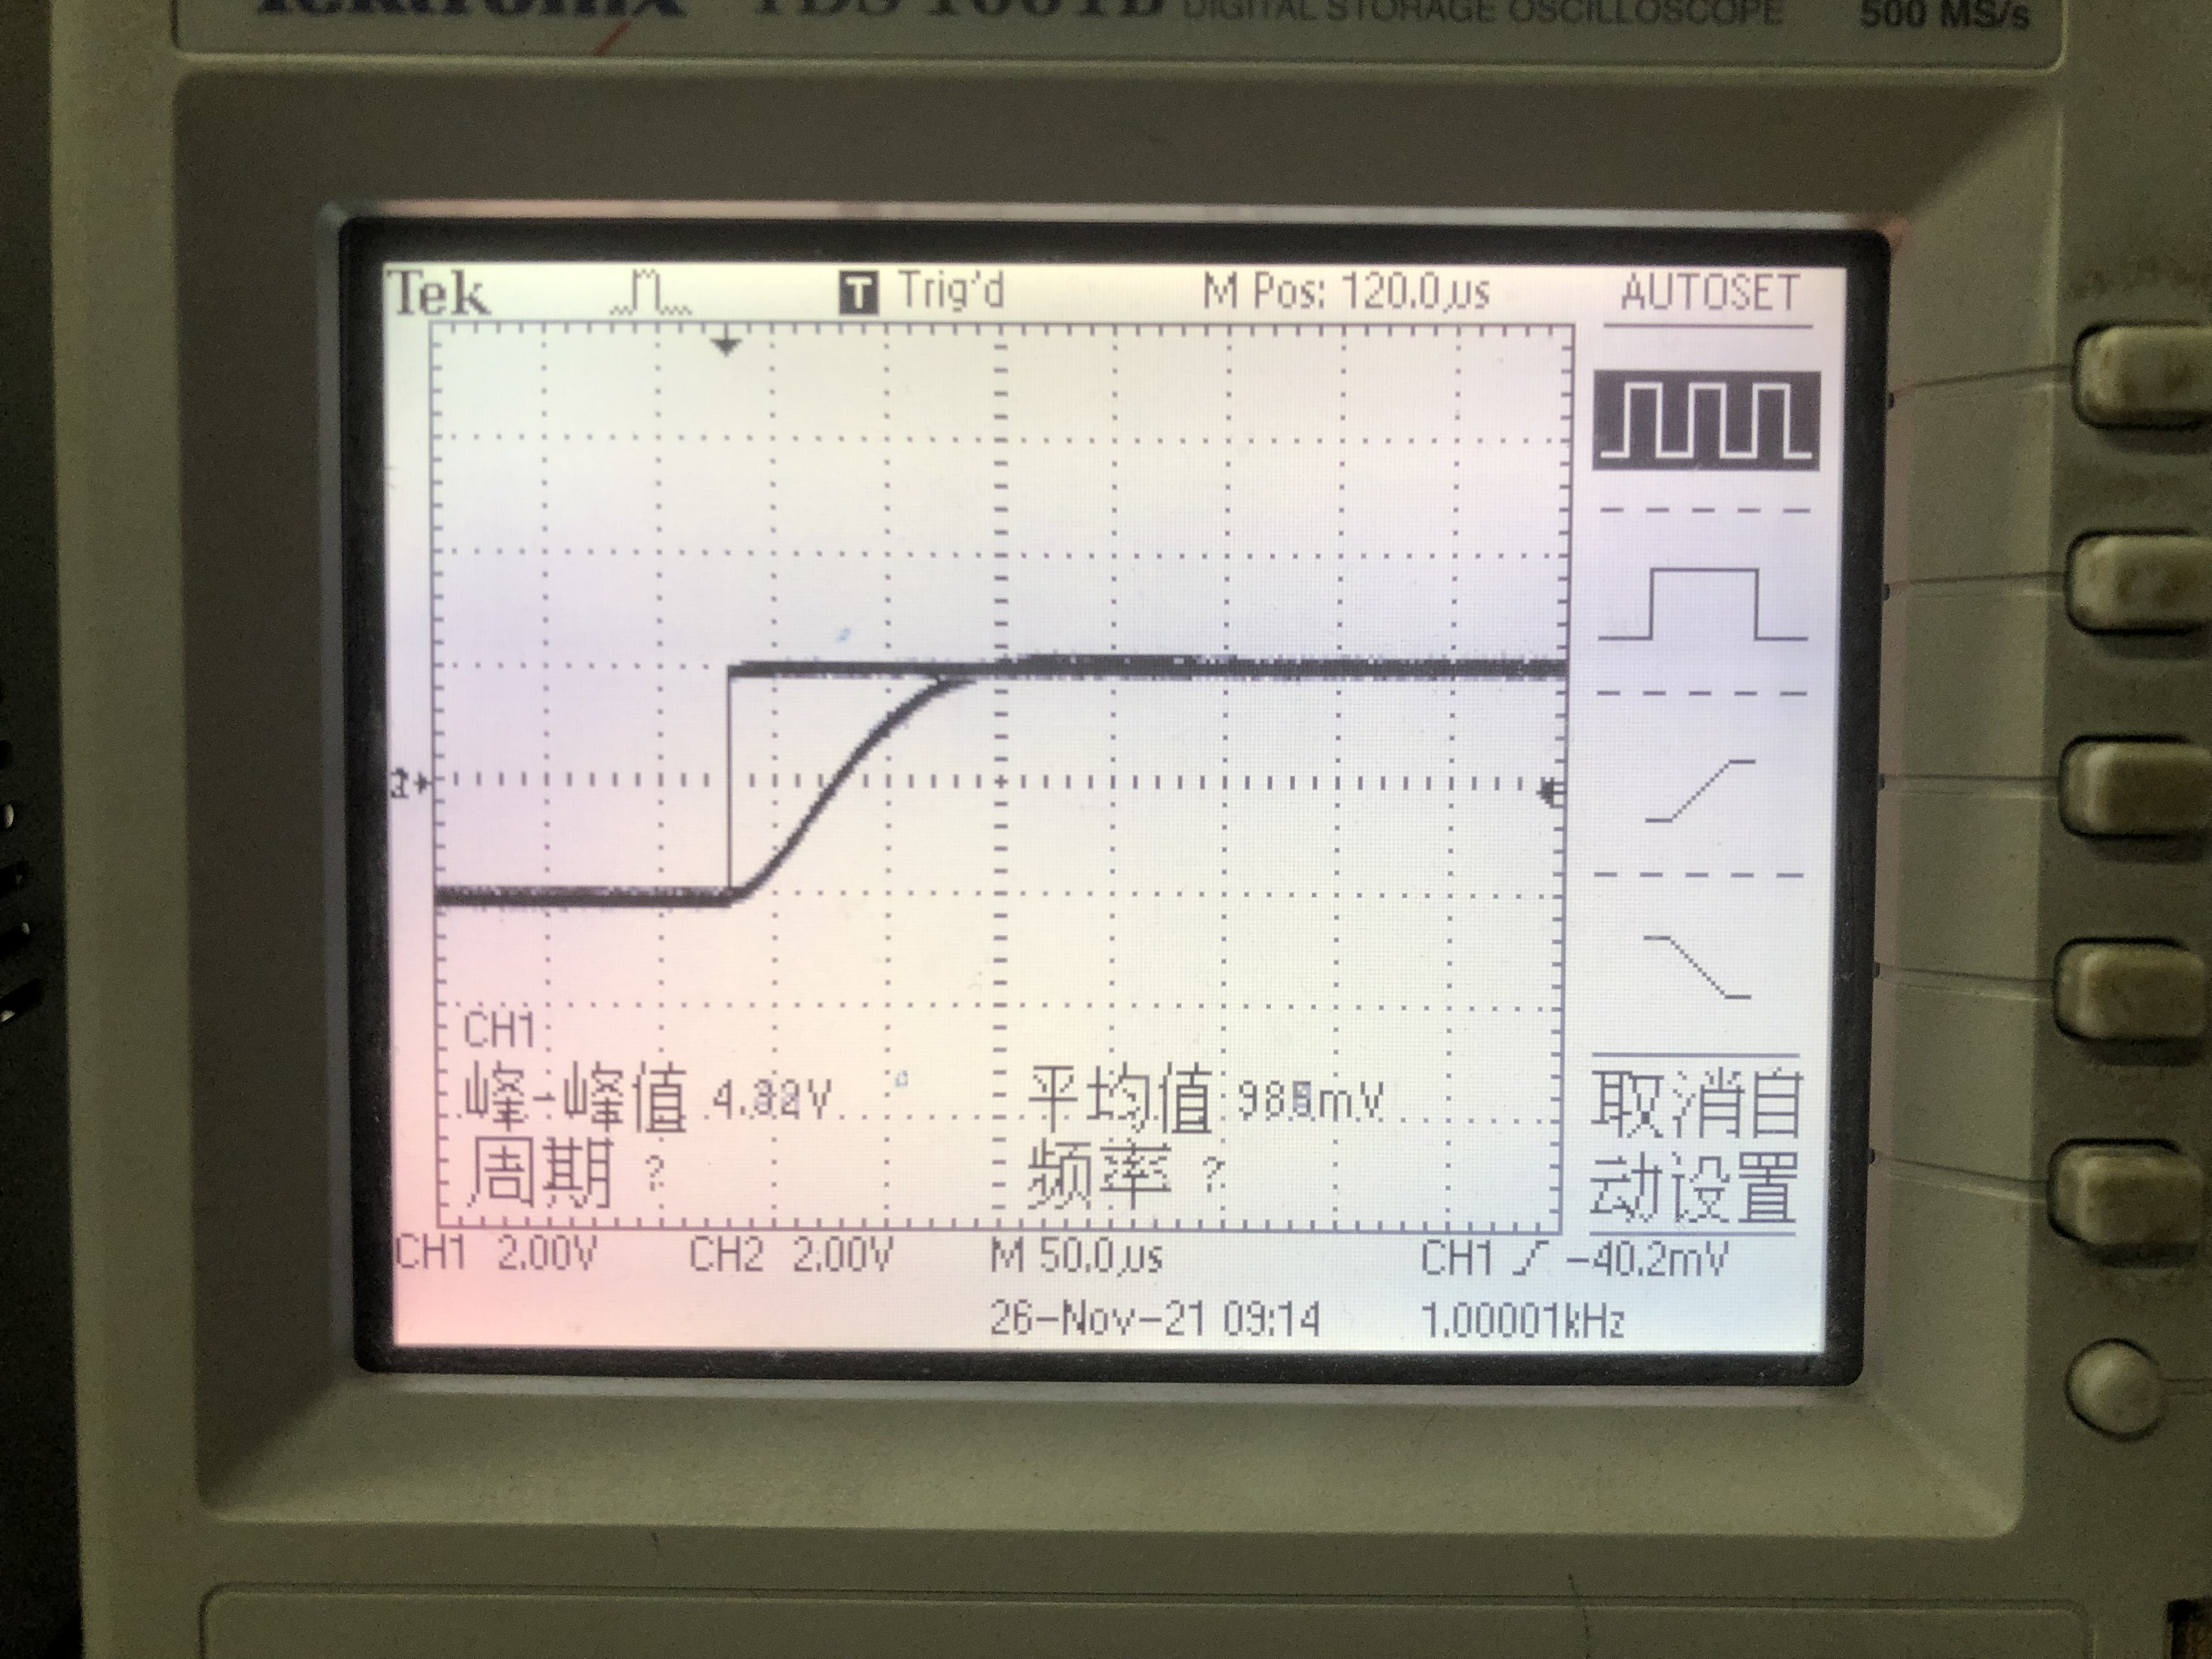
\includegraphics[width=3.5in]{critical}\label{b}
}%

\subfigure[Over-damped regime of the $RLC$ circuit.]{
\centering
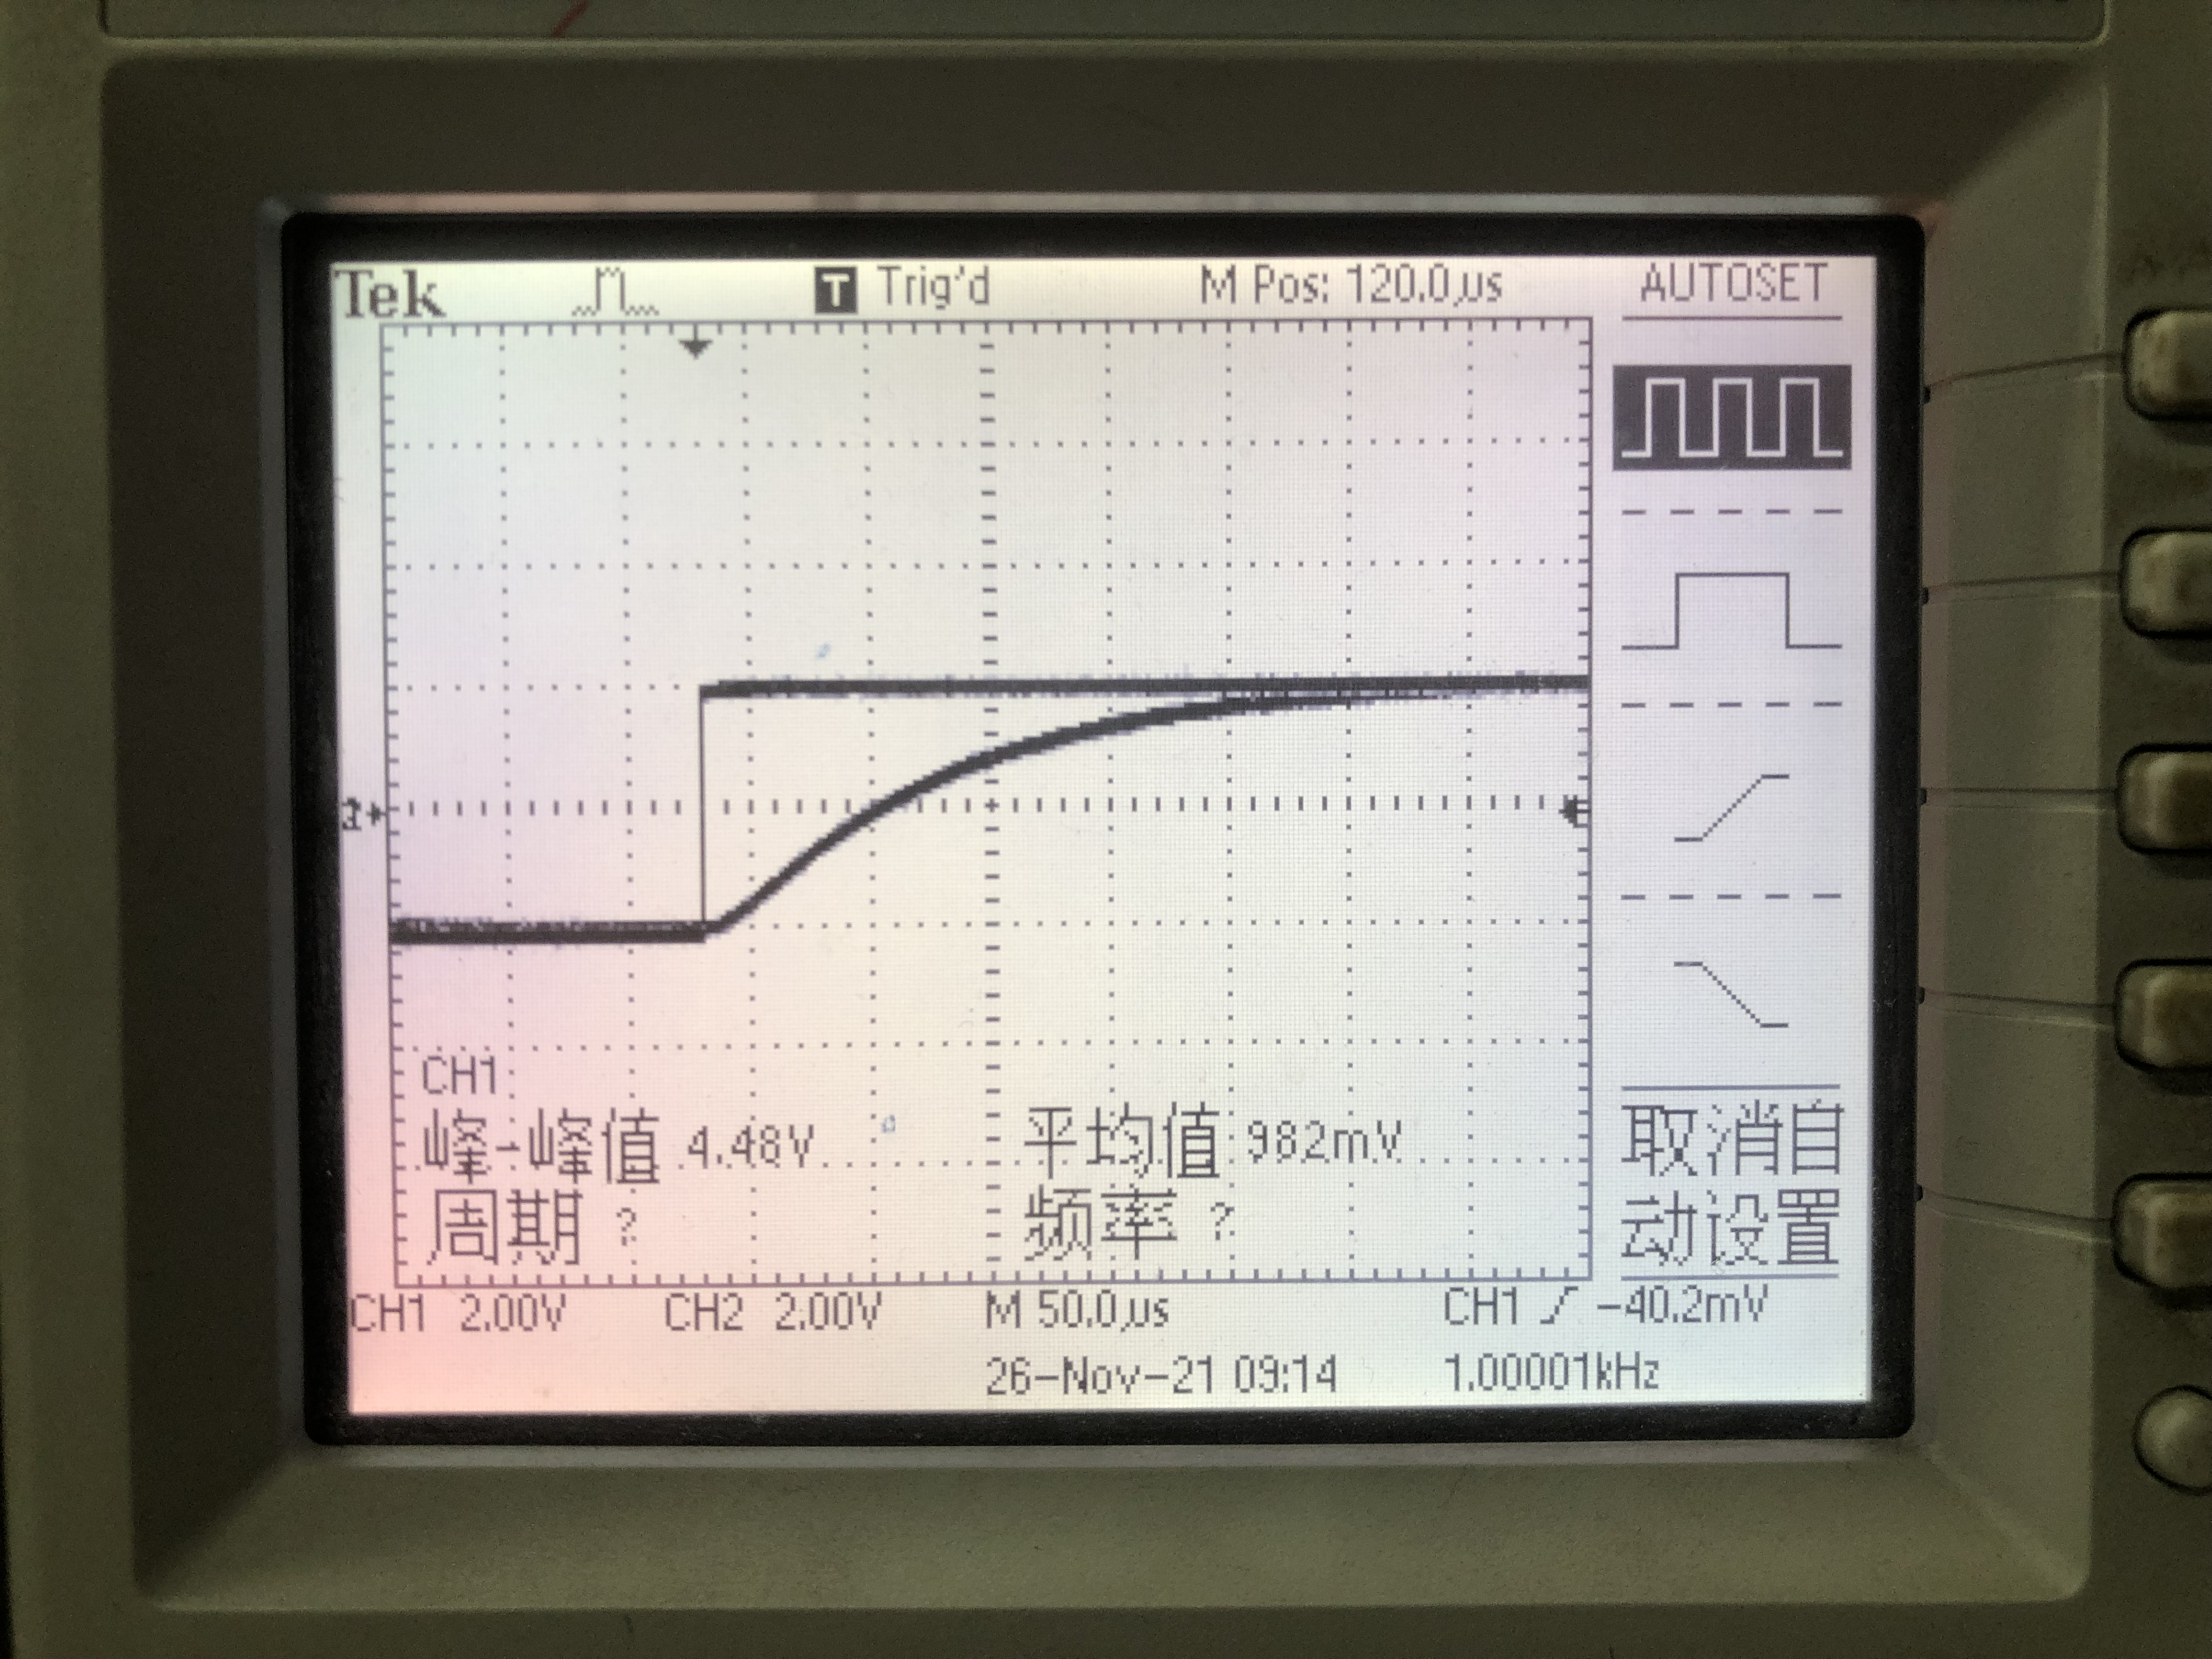
\includegraphics[width=3.5in]{over}\label{c}
}%
\caption{Wave forms of the $RLC$ series circuit. }\label{RLCwave}
\end{figure}


\subsection{$RLC$ Resonant Circuit}

\subsubsection{Relation of $I/I_m$ vs. $f/f_0$ and $\varphi$ vs. $f/f_0$}

The measured data for the $RLC$ resonant circuit are shown in Table \ref{TableResonant}.
\begin{table}[H]\centering
 \begin{tabular}{c|c}
    \toprule
            Quantity & Value \\
        \midrule
        $R\,\,[\Omega]$ & 99.75 $\pm$ 0.01 \\        
        $C$ [nF] & 99.84 $\pm$ 0.01 \\
        $L$ [H] & 0.01 $\pm$ 0 \\
        \midrule
        $\mathcal{E}\,\,[\text{V}_{\text{pp}}]$ & 4.000 $\pm$ 0.001    \\
        $f_0\,\,[\text{Hz}]$ & 5029.000 $\pm$ 0.001 \\
    \end{tabular}        
    
        \begin{tabular}{ccc}

        \toprule
 & $U_R\,\,[\text{V}_\text{pp}] \pm 0.02\,[\text{V}_\text{pp}]$          & $f$ [Hz] $\pm$ 0.001 [Hz] \\
        \midrule
1 & 0.39 & 21420.000 \\
2 & 0.78 & 11120.000 \\
3 & 1.17 & 8600.000 \\
4 & 1.56 & 7420.000 \\
5 & 1.95 & 6730.000 \\
6 & 2.34 & 6300.000 \\
7 & 2.73 & 6000.000 \\
8 & 3.12 & 5700.000 \\
9 & 3.51 & 5450.000 \\
10 & 3.66 & 5340.000 \\
11 & 3.90 & 5029.000 \\
12 & 3.66 & 4710.000 \\
13 & 3.51 & 4640.000 \\
14 & 3.12 & 4430.000 \\
15 & 2.73 & 4230.000 \\
16 & 2.34 & 4010.000 \\
17 & 1.95 & 3740.000 \\
18 & 1.56 & 3400.000 \\
19 & 1.17 & 2920.000 \\
20 & 0.78 & 2180.000 \\
21 & 0.39 & 1900.000 \\
        \bottomrule
    \end{tabular}
    \caption{Measurement data for the $U_R$ vs. $f$ dependence for a $RLC$ resonant circuit.}\label{TableResonant}
\end{table}

To study the properties of resonance, $I/I_m$ vs. $f/f_0$ and $\varphi$ vs. $f/f_0$ plots are needed. 

To get the values of $I/I_m$, $f/f_0$, and $\varphi$, take the first set of data as an example,
$$f/f_0 = \frac{21420.000}{5029.000} = 4.259 \pm 0.0000002,$$
$$I/I_\text{m} = U_R/U_\text{m} = \frac{0.39}{3.90} = 0.100 \pm 0.0014,$$

Note that $\phi$ has two calculation paths, denote them as theoretical value $\varphi_{theo}$ and experimental value $\varphi_{exp}$, respectively, then,
\begin{align*}
    \varphi_{theo} & = \tan^{-1}\bigg(\frac{2\pi fL - \frac{1}{2\pi fC}}{R}\bigg)                                                                 \\
                   & = \tan^{-1}\bigg(\frac{2\pi\times 21420.000\times 0.01-\frac{1}{2\pi \times 21420.000\times 99.84\times10^{-9}}}{99.75}\bigg) \\
                   & = 1.4925 \pm 0.00003 \,[\text{rad}],
\end{align*}
$$
\varphi_\text{exp} = \cos^{-1}\frac{U_R}{U_m} = \cos^{-1}\frac{0.920}{3.90} = 1.3263 \pm 0.0014 \,[\text{rad}],
$$

The rest of the results are shown in Table \ref{TablePhi} below.

\begin{table}[H]\centering
    \begin{tabular}{c|cc|cc|cc|cc}
        \toprule
           &   $I/I_\text{m}$ & $u_{I/I_\text{m}}$ &    $f/f_0$ & $u_{f/f_0}$ & $\varphi_\text{theo}\,[\text{rad}]$ & $u_{\varphi_\text{theo}}\,[\text{rad}]$ & $\varphi_\text{exp}\,[\text{rad}]$ & $u_{\varphi_\text{exp}}\,[\text{rad}]$\\
        \midrule
1 & 0.100 & 0.005 & 4.2592961 & 0.0000009 & 1.4925 & 0.0008 & 1.471 & 0.005 \\
2 & 0.200 & 0.005 & 2.2111752 & 0.0000005 & 1.393 & 0.002 & 1.369 & 0.005 \\
3 & 0.300 & 0.005 & 1.7100815 & 0.0000004 & 1.297 & 0.003 & 1.266 & 0.006 \\
4 & 0.400 & 0.006 & 1.4754424 & 0.0000004 & 1.193 & 0.003 & 1.159 & 0.006 \\
5 & 0.500 & 0.006 & 1.3382382 & 0.0000003 & 1.079 & 0.004 & 1.047 & 0.007 \\
6 & 0.600 & 0.006 & 1.2527341 & 0.0000003 & 0.961 & 0.005 & 0.927 & 0.007 \\
7 & 0.700 & 0.006 & 1.1930801 & 0.0000003 & 0.840 & 0.005 & 0.795 & 0.009 \\
8 & 0.800 & 0.007 & 1.1334261 & 0.0000003 & 0.667 & 0.005 & 0.644 & 0.011 \\
9 & 0.900 & 0.007 & 1.0837145 & 0.0000003 & 0.464 & 0.004 & 0.451 & 0.016 \\
10 & 0.938 & 0.007 & 1.0618413 & 0.0000003 & 0.355 & 0.003 & 0.353 & 0.020 \\
11 & 1.000 & 0.007 & 1.0000000 & 0.0000003 & -0.0100 & 0.0003 & 0 & / \\
12 & 0.938 & 0.007 & 0.9365679 & 0.0000003 & -0.403 & 0.004 & -0.353 & 0.020 \\
13 & 0.900 & 0.007 & 0.9226486 & 0.0000003 & -0.481 & 0.004 & -0.451 & 0.016 \\
14 & 0.800 & 0.007 & 0.8808908 & 0.0000003 & -0.685 & 0.005 & -0.644 & 0.011 \\
15 & 0.700 & 0.006 & 0.8411215 & 0.0000003 & -0.839 & 0.005 & -0.795 & 0.009 \\
16 & 0.600 & 0.006 & 0.7973752 & 0.0000003 & -0.970 & 0.005 & -0.927 & 0.007 \\
17 & 0.500 & 0.006 & 0.7436866 & 0.0000002 & -1.090 & 0.004 & -1.047 & 0.007 \\
18 & 0.400 & 0.006 & 0.6760787 & 0.0000002 & -1.198 & 0.003 & -1.159 & 0.006 \\
19 & 0.300 & 0.005 & 0.5806323 & 0.0000002 & -1.302 & 0.003 & -1.266 & 0.006 \\
20 & 0.200 & 0.005 & 0.4334858 & 0.0000002 & -1.404 & 0.002 & -1.369 & 0.005 \\
21 & 0.100 & 0.005 & 0.3778087 & 0.0000002 & -1.4331 & 0.0014 & -1.471 & 0.005 \\
        \bottomrule
    \end{tabular}
    \caption{Results for $\varphi$, $f/f_0$ and $I/I_\text{m}$.}\label{TablePhi}
\end{table}

Using \textbf{Origin}, the $I/I_\text{m}$ vs. $f/f_0$ and $\varphi_{\text{theo}},\varphi_\text{ex}$ vs. $f/f_0$ curves are plotted in Figure \ref{FigIIm} and Figure \ref{FigPhi}.

\begin{figure}[H]\centering
    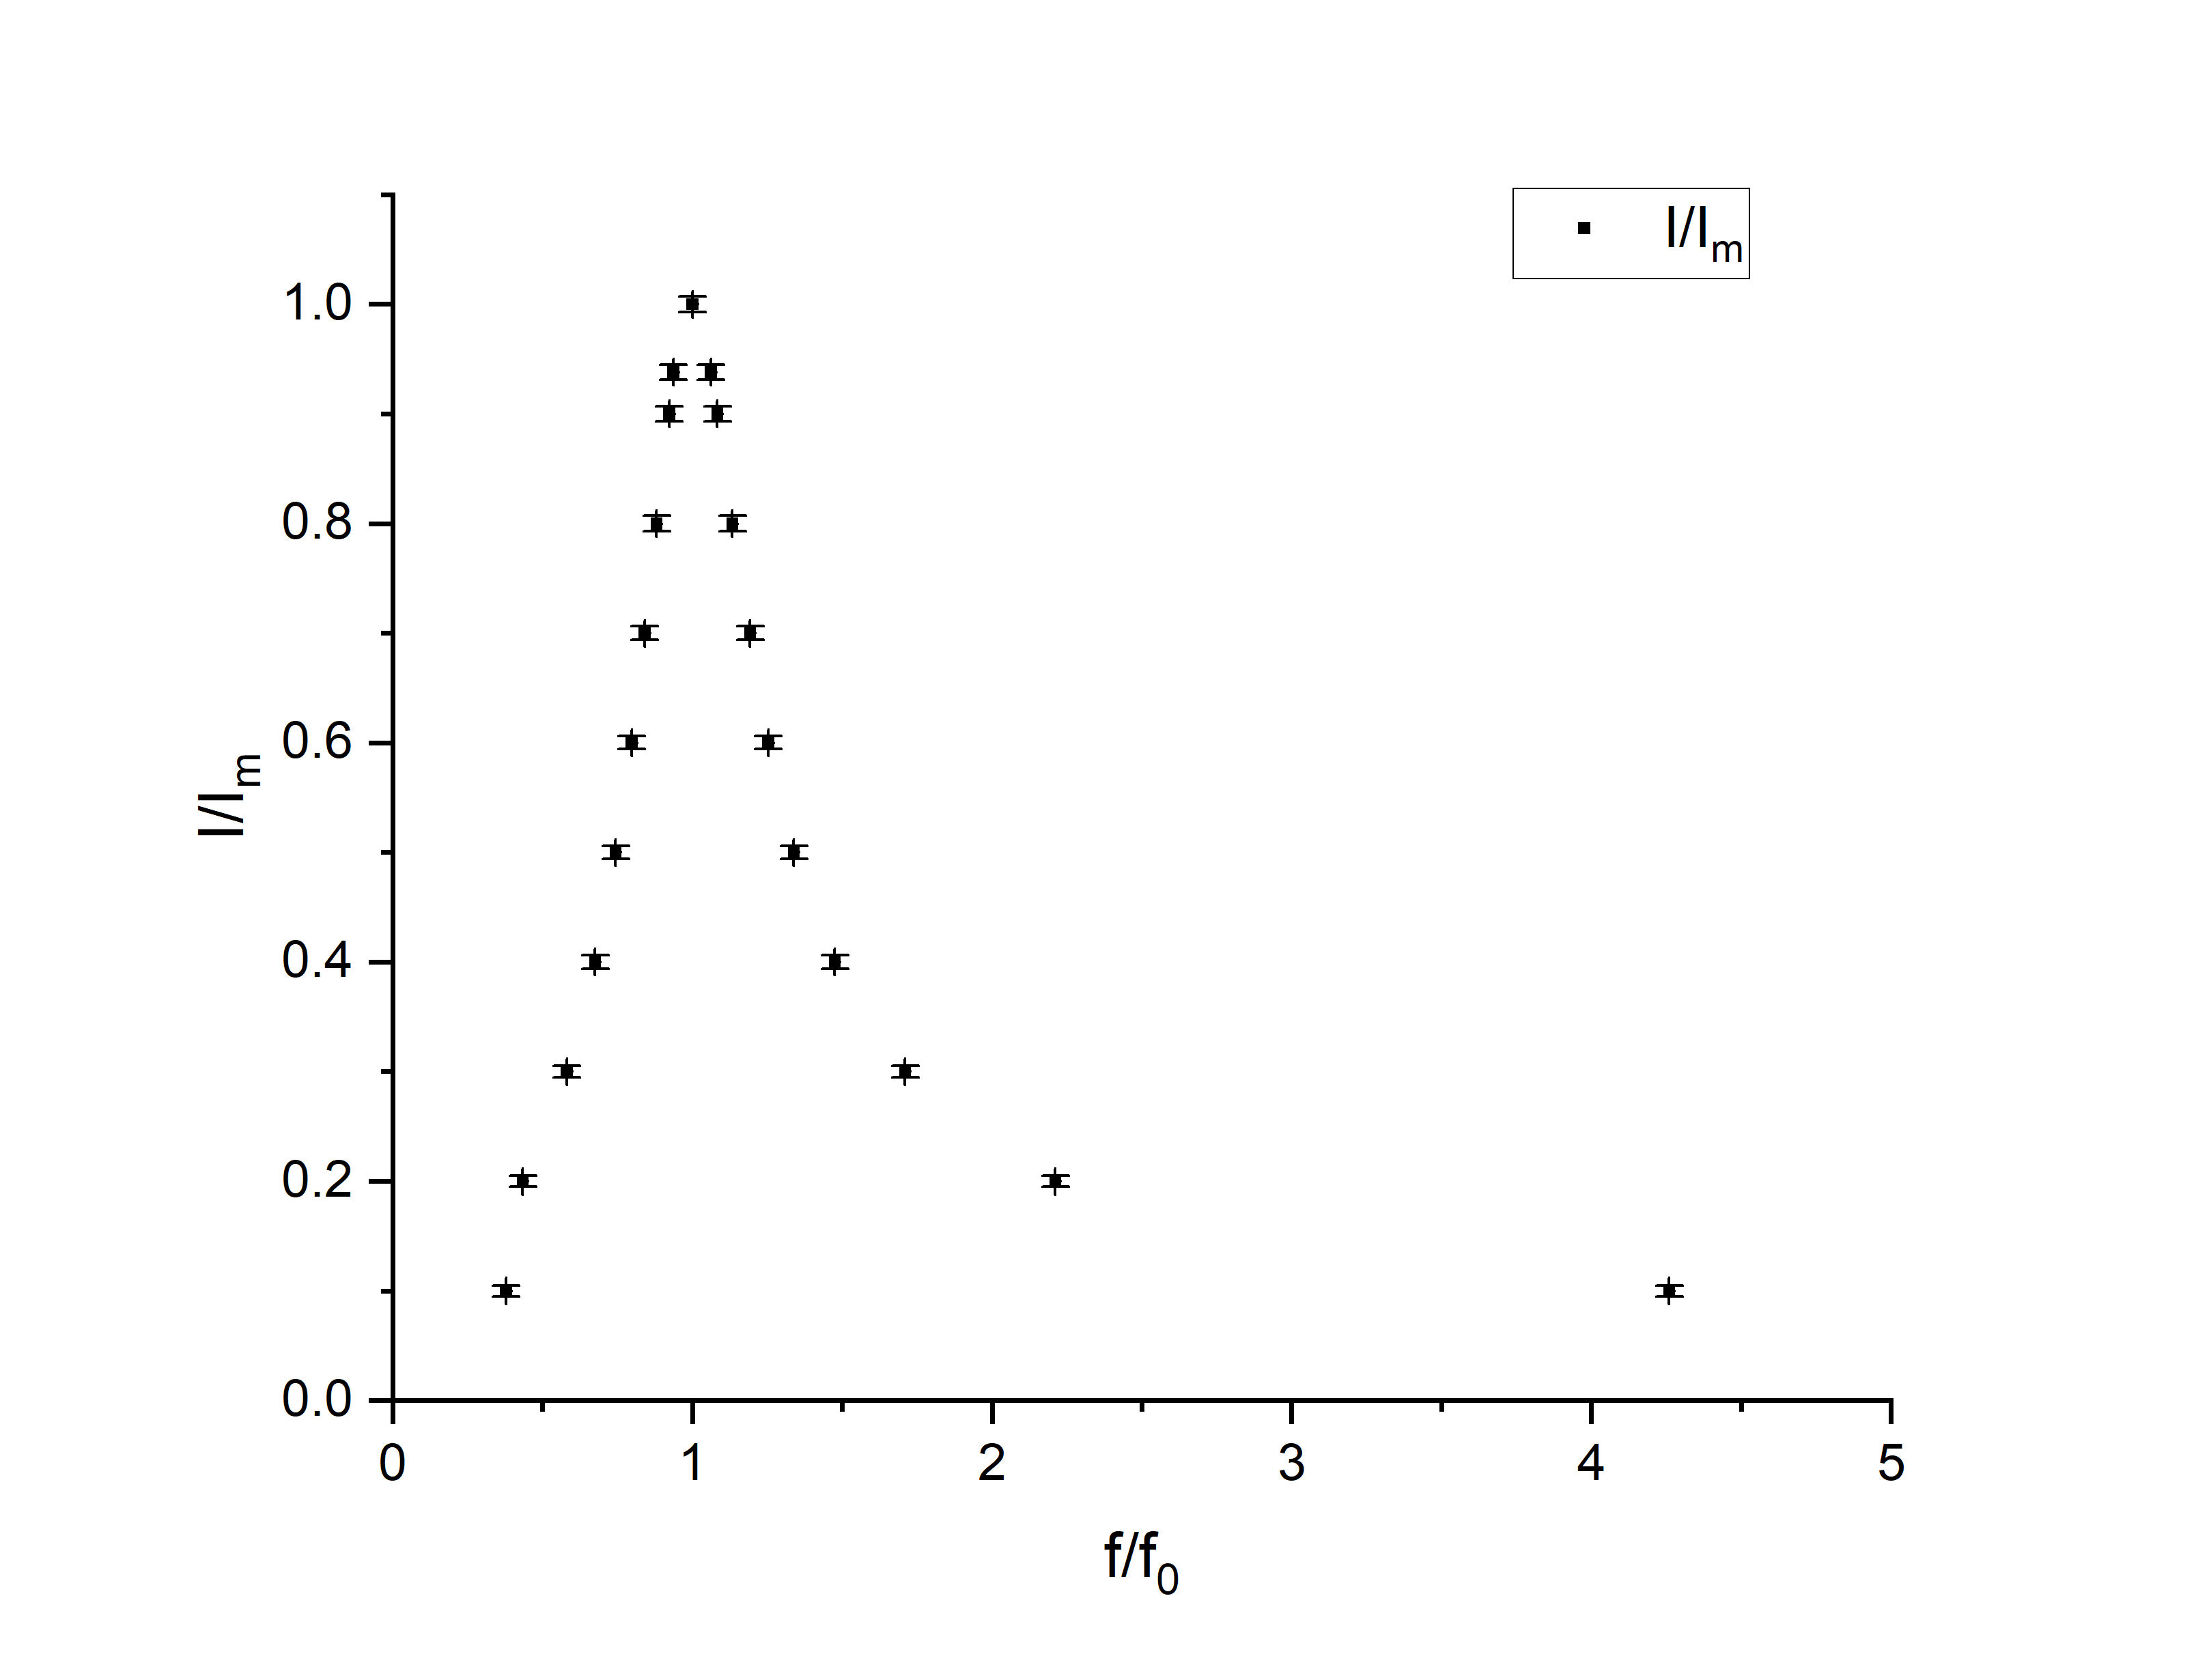
\includegraphics[scale=0.5]{I-f.png}
    \caption{$I/I_\text{m}$ vs. $f/f_0$ relation.}\label{FigIIm}
\end{figure}

\begin{figure}[H]\centering
    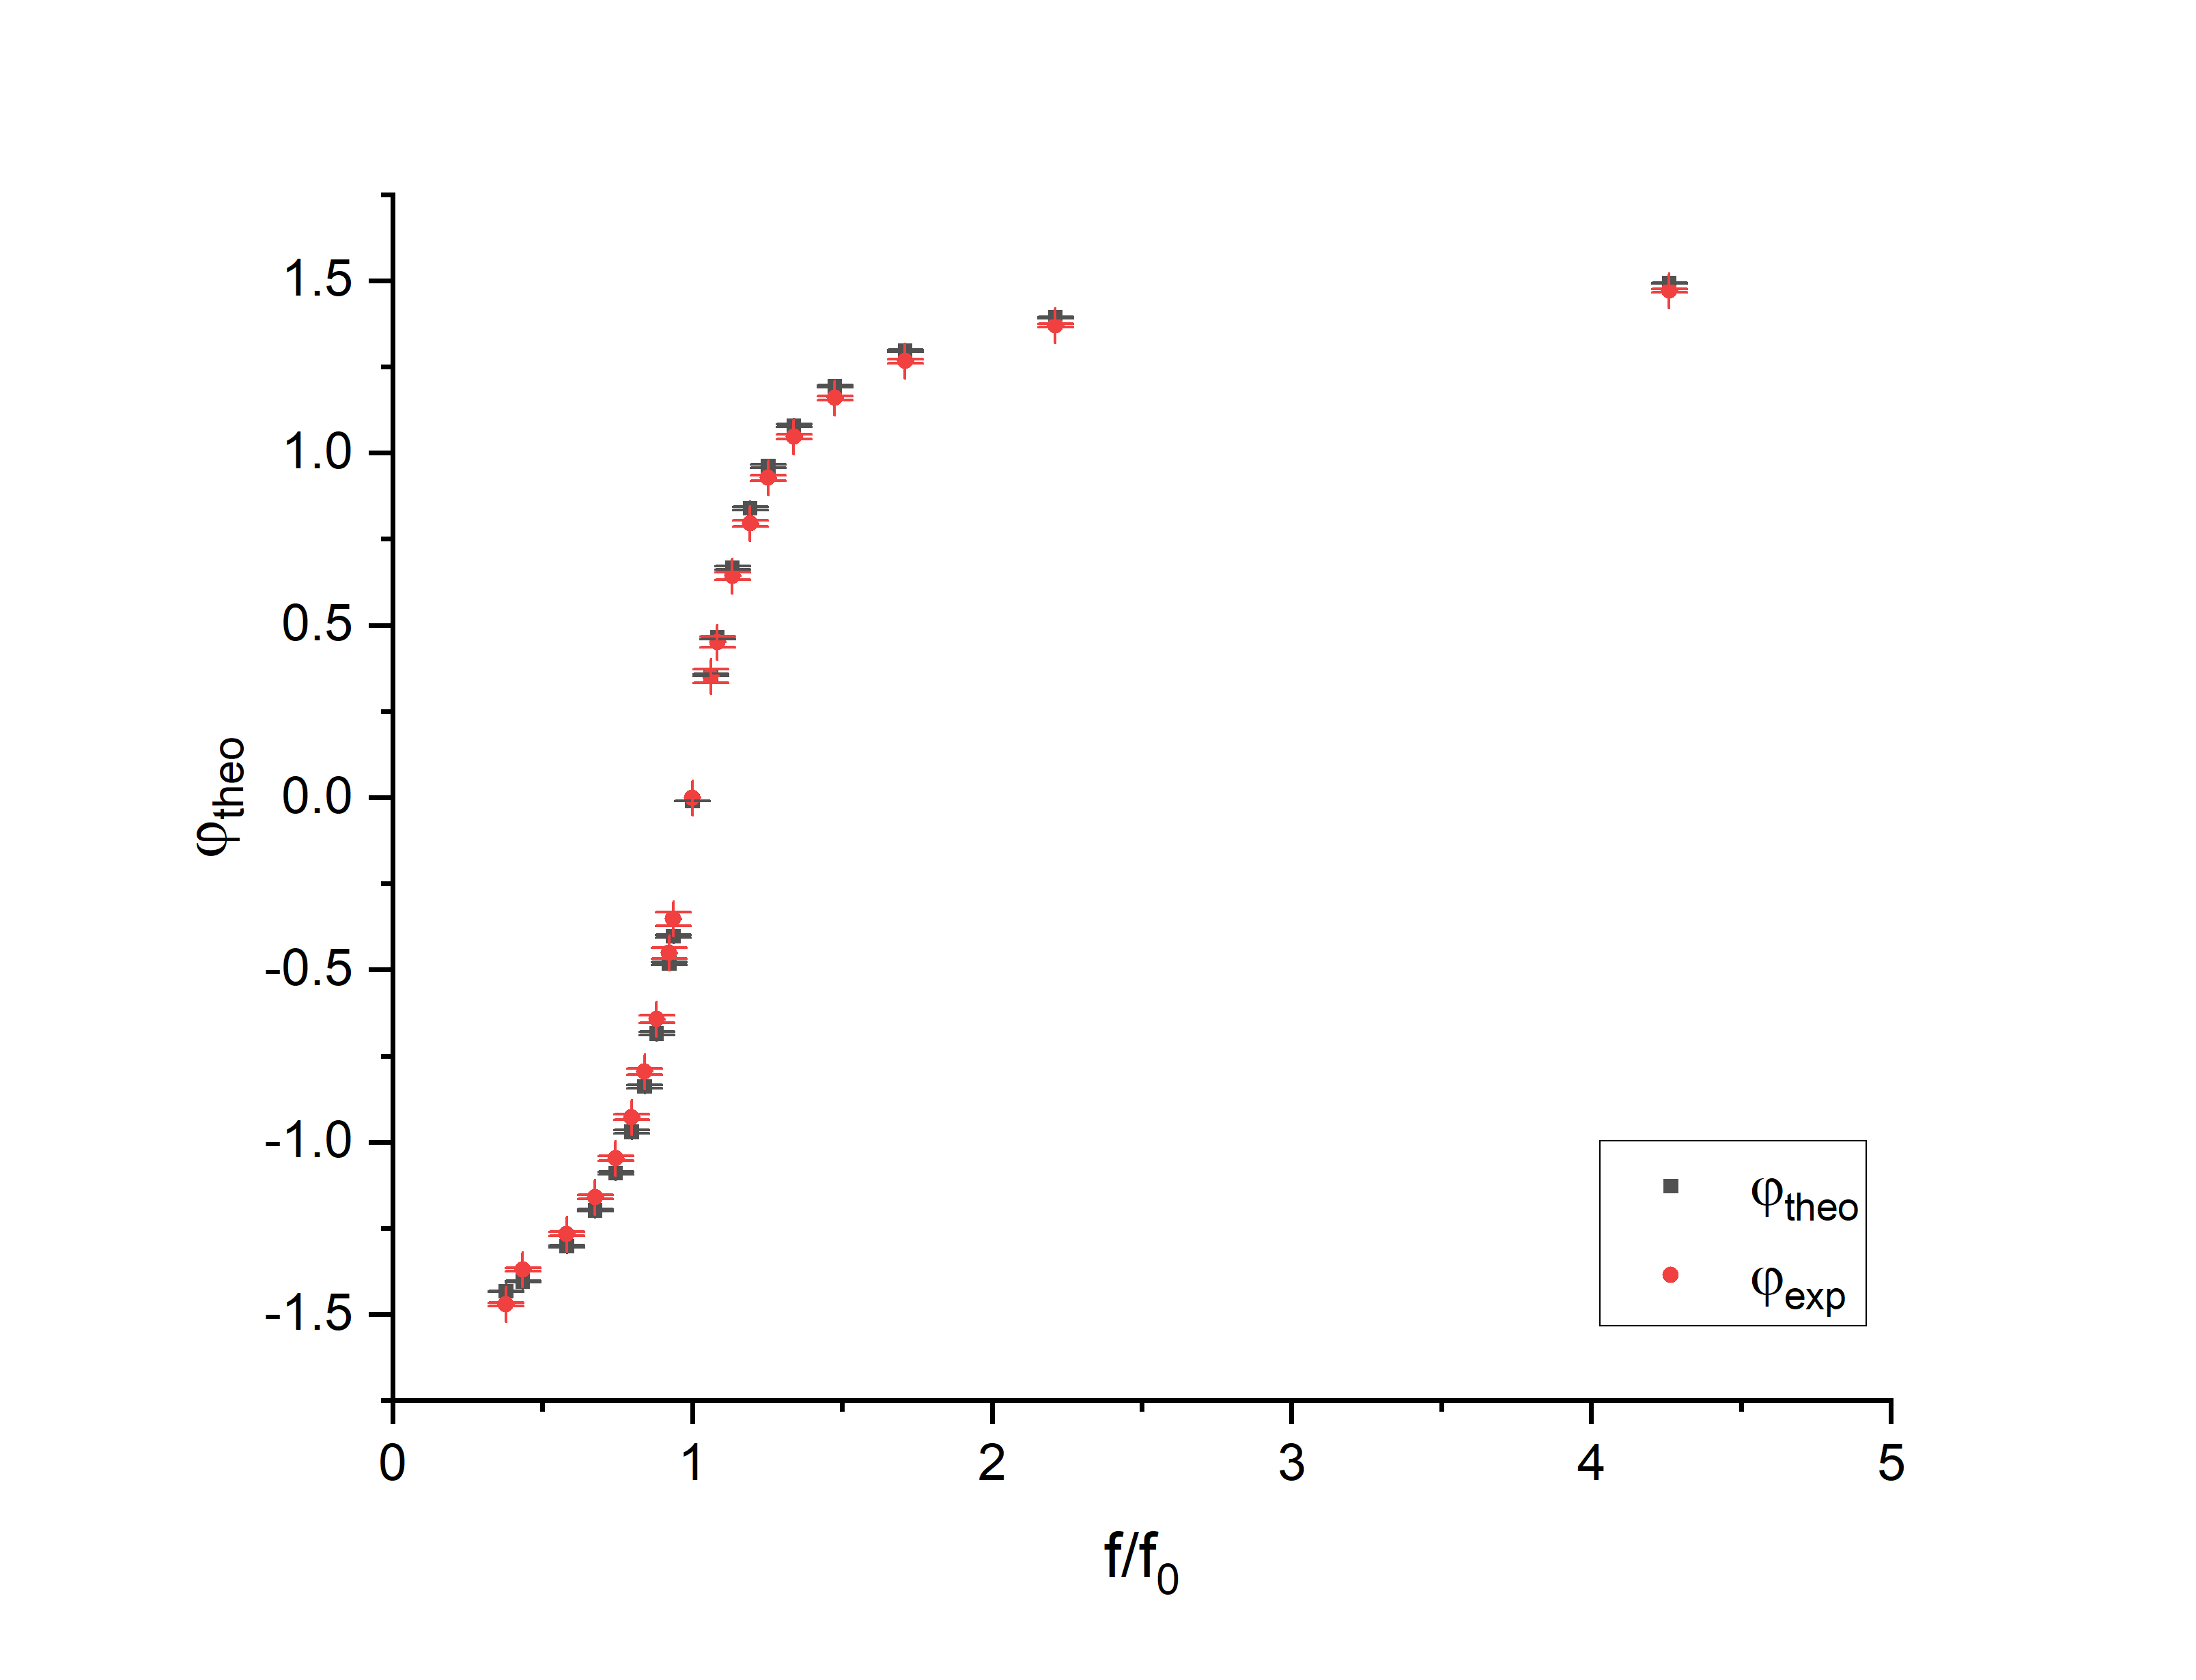
\includegraphics[scale=0.5]{RLC.png}
    \caption{$\varphi$ vs. $f/f_0$ relation.}\label{FigPhi}
\end{figure}



\subsubsection{Quality Factor $Q$}

The experimentally resonance frequency is $f_0 = 5029.000\pm 0.001\,[\text{Hz}]$. According to Eq.\eqref{eq:fres}, the theoretical resonance frequency is

$$f_{0_{theo}} = \frac{1}{2\pi\sqrt{LC}} = \frac{1}{2\pi \sqrt{0.01\times 99.84\times 10^{-9}}} = 5037.0\pm 0.3\,[\text{Hz}]$$

The relative deviation is then
$$u_{r} = \frac{|f_0 - f_{0_{\text{theo}}}|}{f_{0_{\text{theo}}}} \times 100\% = \frac{5037.0 - 5029.000}{5037.0} \times 100\% = 0.16\,\%.$$

According to Eq. \eqref{eq:Qex}, to find the quality factor $Q$, we first need to find out two frequencies $f_1$, $f_2$ such that $I/I_m \approx 1/\sqrt{2}$. Searching Table \ref{TableResonant} and \ref{TablePhi}, we obtain that $f_1 = 4230 \text{Hz}$ and $f_2 = 6000 \text{Hz}$. Then, the theoretical quality factor $Q_{exp}$ can be found as
$$Q_{\text{exp}} = \frac{f_0}{f_2 - f_1} = \frac{5029.000}{6000.000-4230.000} = 2.841243 \pm 0.000002.$$

On the other hand, according to Eq.\eqref{eq:Qtheo}, the theoretical quality factor $Q_{theo}$ can be found as
$$Q_{\text{theo}} = \frac{\sqrt{LC}}{RC} = \frac{\sqrt{0.01\times 99.82\times 10^{-9}}}{100.63\times 99.82\times 10^{-9}} = 3.1727 \pm 0.0003.$$

The relative error is thus
$$u_r = \frac{|Q_{\text{ex}} - Q_{\text{theo}}|}{Q_{\text{theo}}} \times 100\% = \frac{2.841243 - 3.1727}{3.1727} \times 100\% = 10\,\%.$$

\section{Conclusions and Discussion}

\subsection{$RC$, $RL$ and $RLC$ Series Circuits}

In this part, the properties of the wave forms of $RC$, $RL$ and $RLC$ series circuits are studied. \\

As is shown in Figure \ref{RCwave}, when the input voltage changes abruptly at the edge of the square waves, the voltage across the capacitor will not suddenly change. Instead, it will experience exponential saturation until it reaches the input voltage.In steady state, the voltage across the capacitor eventually equals to the source voltage because the capacitor is considered to be open circuit in a DC circuit. 

As is shown in Figure \ref{RLwave}, when the input voltage changes abruptly at the edge of the square waves, the voltage across the resistor in the $RL$ circuit will not suddenly change. As the current is directly proportional to the voltage across the resistor, we may conclude that the current in this circuit experiences exponential saturation. In steady state, the voltage across the resistor eventually equals to the source voltage because the inductor is considered to be no resistance in a DC circuit. 

As is shown in Figure \ref{RLCwave}, when the circuit is underdamped, the voltage across the capacitor will oscillate before going to stability with decreasing amplitude (Figure \ref{a}). When the circuit is critically damped, the voltage goes to stability rapidly (Figure \ref{b}), and if increasing the rheostat, it will turn into underdamped regime.When the circuit is overdamped, the voltage goes to stability just like to wave form of the critically damped circuit. However, the critically damped circuit will go to steady state faster compared with the overdamped circuit (Figure \ref{c}).\\

Then about the time constant, the theoretical time constants and experimental tie constants of the three regime are compiled together in Table \ref{TableResult} below:

\begin{table}[H]\centering
    \begin{tabular}{cccc}
        \toprule
                      & Experimental $\tau\,\,[\mu\text{s}]$ & Theoretical $\tau_{\text{theo}}\,\,[\mu\text{s}]$ & Relative error \\
        \midrule
        $RC$ circuit  & 10.0989 $\pm$ 0.0014                 & 9.9590 $\pm$ 0.0014                              & 1.4$\%$      \\
        $RL$ circuit  & 95.218 $\pm$ 0.014                  & 103.874 $\pm$ 0.010                                & 5$\%$       \\
        $RLC$ circuit & 30.00 $\pm$ 0.01                     & 31.5943 $\pm$ 0.0016                              & 5$\%$      \\
        \bottomrule
    \end{tabular}
    \caption{Result of time constant in $RC$, $RL$ and $RLC$ series circuits.}\label{TableResult}
\end{table}

In general, three circuits' experimental results are close to the theoretical ones with acceptable errors. 

Still, the minor errors may comes from the inaccuracy of the oscilloscope. When I was trying to shift the cursor so that the voltage difference reaches a certain value, due to the instability of the voltage, it is hard to precisely hit the expected point exactly, causing errors.

\subsection{$RLC$ Resonant Circuit}

In the second part of the experiment, the $RLC$ resonance circuit are studied. \\

Figure \ref{FigIIm} shows the amplitude-frequency relation. From the figure, we can see that the amplitude maximized at resonance frequency, and decreases on the other sides. Then we can infer that when $f \rightarrow 0$, the current would  approach 0; and as $f\rightarrow \infty$, the current would also approach 0.

Figure \ref{FigPhi} compares the theoretical and experimental phase differences in frequency domain. Both of them match the shape of the function of $arctangent$. And the two curves are quite close. In general, the phase difference matches with theory quite well.\\

The experimental and theoretical results of resonance frequency $f_0$ and quality factor $Q$ are summarized in Table Table \ref{tab:fQ}.

\begin{table}[H] \centering
    \begin{tabular}{cccc}
        \toprule
                           & Experimental           & Theoretical        & Relative error \\
        \midrule
        $f_0\,[\text{Hz}]$ & $5029.000\pm 0.001$    & $5037.0\pm 0.2$    & 0.16\%             \\
        $Q$                & $2.841243\pm 0.000003$ & $3.1727\pm 0.0004$ & 10\%         \\
        \bottomrule
    \end{tabular}
    \caption{Result of resonance frequency and quality factor.}
    \label{tab:fQ}
\end{table}

The experimental result of the resonance frequency is quite close to the theoretical one, which can be considered to be successful.

However, the experimental result of the quality factor is not that satisfying, with relative errors up to 10\%. The possible reasons for such big error are listed below:
\begin{enumerate}
\item Theoretically, we need to choose two frequencies $f_1$, $f_2$ such that $I/I_m = 1/\sqrt{2}$. However, there is no set of data measured exactly at the point $I/I_m = 1/\sqrt{2}$ and we can only choose the data most close to that point, whose deviation causing errors.
\item When the frequency gets farther from the resonance frequency, the voltage becomes less sensitive to the changing frequency. Therefore the two frequencies chosen might not be that accurate, causing errors.
\end{enumerate}

\subsection{Suggestions and Improvement}

The following suggestions may help to improve the experiment:
\begin{enumerate}
\item If possible, replace the oscilloscope with one with high resolution like what we use in VE215's lab. 
 \item Otherwise, the measured value of $U_R$ is not stable, one possible solution is to measure the values for more times, for instance, 3 times, and take the averages as results.
 \item To find the quality factor $Q$ more precisely, I suggest to calculate the theoretical value first and then set the frequencies based on the theoretical voltage (current). In this way we can directly get the data point we need to use in the calculation of quality factor.
\end{enumerate}

\subsection{Conclusions}

In this lab, the waveforms of the $RC$, $RL$ and $RLC$ series circuits are studied and the corresponding time constants are found out. Then,  the resonance phenomenon is studied. The corresponding curves are plotted using Origin and the resonance frequency and the quality factor is estimated. Most of the results got in the experiment are close to the theoretical ones. In general, the objectives of lab are fulfilled.

\begin{thebibliography}{1}

    \bibitem{manual} VP241 Exercise 5: RC, RL, and RLC Circuits, UM-SJTU Joint Institute.

\end{thebibliography}

\newpage

\appendix

\section{Uncertainty Analysis}

\subsection{$RC$ Circuit}
The experimental value of the time constant is given by 
\[\tau=\frac{T_{1/2}}{\ln 2}.\] 
So, the uncertainty is 
\[u_{\tau}=\left|\frac{\rm d}{\rm d (T_{1/2})}\left(\frac{T_{1/2}}{\ln 2}\right)u_{T_{1/2}}\right|=\frac{u_{T_{1/2}}}{\ln 2}.\] 
Here the uncertainty of $T_{1/2} $ is 0.001$[\mu$s], so the uncertainty of $\tau$ is 
\[u_{\tau}=\frac{0.001}{\ln 2}=0.0014[\mu \rm s]\]

The theoretical value of the time constant is given by 
\[\tau_{\rm theo}=RC.\] 
So the uncertainty is 
\[u_{\tau_{theo}}=\sqrt{\left(\frac{\partial}{\partial R}(RC)u_R\right)^2+\left(\frac{\partial}{\partial C}(RC)u_C\right)^2}=\sqrt{C^2u_R^2+R^2u_C^2}.\] 
Here the parameters are given as \(R=99.75\Omega, C=9.984\times 10^{-8}{\rm F}, u_C=10^{-11}{\rm F}, u_R=0.01\Omega\), which yield
\[u_{\tau_{theo}}=0.10[\mu s]\].

\subsection{$RL$ Circuit}
The experimental value of the time constant is given by 
\[\tau=\frac{T_{1/2}}{\ln 2}.\] 
So, the uncertainty is 
\[u_{\tau}=\left|\frac{\rm d}{\rm d (T_{1/2})}\left(\frac{T_{1/2}}{\ln 2}\right)u_{T_{1/2}}\right|=\frac{u_{T_{1/2}}}{\ln 2}.\] 
Here the uncertainty of $T_{1/2} $ is 0.01$[\mu$s], so the uncertainty of $\tau$ is 
\[u_{\tau}=\frac{0.01}{\ln 2}=0.014[\mu \rm s]\]

The theoretical value of the time constant is given by 
\[\tau_{\rm theo}=\frac{L}{R}.\] 
So the uncertainty is 
\[u_{\tau_{theo}}=\sqrt{\left(\frac{\partial}{\partial R}\left(\frac{L}{R}\right)u_R\right)^2+\left(\frac{\partial}{\partial L}\left(\frac{L}{R}\right)u_L\right)^2}=\sqrt{\frac{u_L^2}{R^2}+\frac{L^2u_R^2}{R^4}}.\] 
Here the parameters are given as \(R=99.75\Omega,L=0.01{\rm H},u_R=0.01\Omega,u_L=0\), which yield
 \[u_{\tau_{theo}}=0.010[\mu \rm s].\]

\subsection{Uncertainty of Data for $RLC$ Circuit}
The experimental value of the time constant is given by 
\[\tau=\frac{T_{0.264}}{1.00}.\] 
So, the uncertainty is 
\[u_{\tau}=\left|\frac{\rm d}{\rm d (T_{0.264})}\left(\frac{T_{0.264}}{1.00}\right)u_{T_{0.254}}\right|=\frac{u_{T_{1/2}}}{1.00}.\] 
Here the uncertainty of $T_{0.264} $ is 0.01$[\mu$s], so the uncertainty of $\tau$ is 
\[u_{\tau}=\frac{0.01}{1.00}=0.010[\mu \rm s]\]

The theoretical value of the time constant is given by 
\[\tau_{\rm theo}=\sqrt{LC}.\] 
But the uncertainty of $L$ is equal to 0, the uncertainty can be simplified as 
\[u_{\tau_{theo}}=\left|\frac{\partial}{\partial C}(\sqrt{LC})u_C\right|=\frac{\sqrt{L}u_C}{2\sqrt{C}}.\] 
Here $L=0.01{\rm H},C=99.84{\rm nF}, u_C=0.01{\rm nF}$, which yield
\[u_{\tau_{theo}}=0.0016[\mu s].\]

\subsection{$RLC$ Resonant Circuit}

\subsubsection{$f/f_0$}

For $f/f_0$, the uncertainty is given by
$$u_{f/f_0} = \sqrt{(\frac{\partial f/f_0}{\partial f}u_f)^2 + (\frac{\partial f/f_0}{\partial f_0}u_{f_0})^2} = \sqrt{(\frac{u_f}{f_0})^2 + (-\frac{f}{f_0^2}u_{f_0})^2}.$$

Take the first set of data as an example,

\begin{align*}
    u_{f/f_0} & = \sqrt{(\frac{u_f}{f_0})^2 + (-\frac{f}{f_0^2}u_{f_0})^2}                         \\
              & = \sqrt{(\frac{0.001}{5029.000})^2 + (-\frac{21420.000}{5029.000^2}\times 0.001)^2} \\
              & = 0.0000009.
\end{align*}

The rest of the uncertainties are calculated in the same way and are shown in Table \ref{TablePhi} following the data of $f/f_0$.

\subsubsection{$I/I_m$}
For $I/I_\text{m} = U_R/U_\text{m}$, the uncertainty is given by

$$u_{I/I_\text{m}} = \sqrt{(\frac{\partial U_R/U_\text{m}}{\partial U_R}u_{U_R})^2 + (\frac{\partial U_R/U_\text{m}}{\partial U_\text{m}}u_{U_\text{m}})^2} = \sqrt{(\frac{u_{U_R}}{U_\text{m}})^2 + (-\frac{U_R}{U_\text{m}^2}u_{U_\text{m}})^2}.$$

Take the first set of data as an example,

\begin{align*}
    u_{I/I_\text{m}} & = \sqrt{(\frac{u_{U_R}}{U_\text{m}})^2 + (-\frac{U_R}{U_\text{m}^2}u_{U_\text{m}})^2} \\
                     & = \sqrt{(\frac{0.02}{3.90})^2 + (-\frac{0.39}{3.90^2}\times 0.02)^2}                 \\
                     & = 0.005.
\end{align*}

The rest of the uncertainties are calculated in the same way and are shown in Table \ref{TablePhi} following the data of $I/I_0$.

\subsubsection{$\varphi_\text{theo}$}
For $\varphi_\text{theo} = \tan^{-1}\bigg(\frac{2\pi fL-\frac{1}{2\pi fC}}{R}\bigg)$, the uncertainty is given by 

\begin{align*}
    u_{\varphi_\text{theo}} & = \sqrt{(\frac{\partial \varphi_\text{theo}}{\partial f}u_f)^2 + (\frac{\partial \varphi_\text{theo}}{\partial C}u_C)^2 + (\frac{\partial \varphi_\text{theo}}{\partial R}u_R)^2}                                                                                                                                               \\
                            & = \sqrt{\left( \frac{R\big(2\pi L +\frac{1}{2\pi f^2 C}\big)}{R^2 + \big(2\pi fL - \frac{1}{2\pi fC}\big)^2} u_f \right)^2 + \left( \frac{R}{2\pi fC^2\big[R^2+\big(2\pi fL - \frac{1}{2\pi fC}\big)^2\big]} u_C \right)^2 + \left(-\frac{2\pi fL-\frac{1}{2\pi fC}}{R^2+\big(2\pi fL-\frac{1}{2\pi fC}\big)^2} u_R \right)^2}.
\end{align*}

Take the first set of data as an example,here $f=21429[\rm kHz]$, $L=0.01[\rm H]$, $C=99.84[\rm nF]$, $R=99.75[\Omega]$, $u_C=0.01[\rm nF]$, $u_R=0.01[\Omega]$, $u_f=0.001[\rm Hz]$,which yield
$$u_{\varphi_\text{theo}} = 0.0008$$

The rest of the uncertainties are calculated in the same way and are shown in Table \ref{TablePhi} following the data of $\varphi_{theo}$.


\subsubsection{$\varphi_\text{ex}$}
For $\varphi_\text{exp}=cos^{-1}(\frac{U_R}{U_m})$, the uncertainty is given by

$$u_{\varphi_\text{ex}} = \sqrt{(\frac{\partial \varphi_\text{ex}}{\partial U_R}u_{U_\text{R}})^2 + (\frac{\partial \varphi_\text{ex}}{\partial U_m}u_{U_\text{m}})^2} = \sqrt{(\frac{-1}{\sqrt{U_m^2-U_R^2}}u_{U_\text{R}})^2 + (\frac{U_R}{U_m\sqrt{U_m^2-U_R^2}}u_{U_\text{m}})^2}.$$

Take the first set of data as an example,here $u_U=0.012[\rm V]$, $U_m=3.90[\rm V]$, $U_R=0.39[\rm V]$, which yield
$$u_{\varphi_\text{exp}} = 0.005$$

The rest of the uncertainties are calculated in the same way and are shown in Table \ref{TablePhi} following the data of $\varphi_{exp}$.

\newpage 
Here provides a table of summary of the uncertainties in this part.

\begin{table}[H]\centering
    \begin{tabular}{ccccc}
        \toprule
           & $u_{f/f_0}$ & $u_{I/I_\text{m}}$ & $u_{\varphi_\text{theo}}\,[\text{rad}]$ & $u_{\varphi_\text{ex}}\,[\text{rad}]$ \\
        \midrule
1 & 0.005 & 0.0000009 & 0.0008 & 0.005 \\
2 & 0.005 & 0.0000005 & 0.002 & 0.005 \\
3 & 0.005 & 0.0000004 & 0.003 & 0.006 \\
4 & 0.006 & 0.0000004 & 0.003 & 0.006 \\
5 & 0.006 & 0.0000003 & 0.004 & 0.007 \\
6 & 0.006 & 0.0000003 & 0.005 & 0.007 \\
7 & 0.006 & 0.0000003 & 0.005 & 0.009 \\
8 & 0.007 & 0.0000003 & 0.005 & 0.011 \\
9 & 0.007 & 0.0000003 & 0.004 & 0.016 \\
10 & 0.007 & 0.0000003 & 0.003 & 0.020 \\
11 & 0.007 & 0.0000003 & 0.0003 & / \\
12 & 0.007 & 0.0000003 & 0.004 & 0.020 \\
13 & 0.007 & 0.0000003 & 0.004 & 0.016 \\
14 & 0.007 & 0.0000003 & 0.005 & 0.011 \\
15 & 0.006 & 0.0000003 & 0.005 & 0.009 \\
16 & 0.006 & 0.0000003 & 0.005 & 0.007 \\
17 & 0.006 & 0.0000002 & 0.004 & 0.007 \\
18 & 0.006 & 0.0000002 & 0.003 & 0.006 \\
19 & 0.005 & 0.0000002 & 0.003 & 0.006 \\
20 & 0.005 & 0.0000002 & 0.002 & 0.005 \\
21 & 0.005 & 0.0000002 & 0.0014 & 0.005 \\
        \bottomrule
    \end{tabular}
    \caption{Uncertainty for $\varphi$, $f/f_0$ and $I/I_\text{m}$.}\label{TableUnc}
\end{table}

\subsubsection{$f_{0_{\text{theo}}}$}

For $f_{0_\text{{theo}}} = \frac{1}{2\pi\sqrt{LC}}$, the uncertainty is given by

\begin{align*}
    U_{f_{0_{\text{theo}}}} & = \sqrt{(\frac{\partial f_{0_{\text{theo}}}}{\partial L}u_L)^2 + (\frac{\partial f_{0_{\text{theo}}}}{\partial C}u_C)^2}                                                                     \\
                            & = \sqrt{\left[\frac{1}{2 \pi \sqrt{C}}\left(-\frac{1}{2} L^{-\frac{3}{2}}\right) u_{L}\right]^{2}+\left[\frac{1}{2 \pi \sqrt{L}}\left(-\frac{1}{2} C^{-\frac{3}{2}}\right) u_{C}\right]^{2}} \\
                            & =\left|\frac{1}{2 \pi \sqrt{L}}\left(-\frac{1}{2} C^{-\frac{3}{2}}\right) u_{C}\right|
\end{align*}

Here $L=0.01[\rm H]$, $C=99.84[\rm nF]$, $u_C=0.01[\rm nF]$,which yield
$$u_{\varphi_\text{theo}} = 0.3$$

\subsubsection{$Q_\text{exp}$}

For $Q_\text{ex} = \frac{f_0}{f_2 - f_1}$, the uncertainty

\begin{align*}
    u_{Q_\text{exp}} & = \sqrt{(\frac{\partial Q_\text{ex}}{\partial f_0}u_{f_0})^2 + (\frac{\partial Q_\text{ex}}{\partial f_1}u_{f_1})^2 + (\frac{\partial Q_\text{ex}}{\partial f_2}u_{f_2})^2}                 \\
                    & = \sqrt{\bigg(\frac{u_{f_0}}{f_2-f_1}\bigg)^2 + \bigg(\frac{f_0}{(f_2-f_1)^2}u_{f_1}\bigg)^2 + \bigg(-\frac{f_0}{(f_2-f_1)^2}u_{f_2}\bigg)^2}                                                                                       
\end{align*}

Here $f_0 = 5029 [\rm Hz]$, $f_1 = 4230 [\rm Hz]$,$f_0 = 6000 [\rm Hz]$,which yield
$$u_{Q_\text{exp}} = 0.000002$$

\subsubsection{$Q_\text{theo}$}

For $Q_\text{theo} = \frac{\sqrt{LC}}{RC}$, the uncertainty is given by

\begin{align*}
    u_{Q_{\text{theo}}} & = \sqrt{(\frac{\partial Q_{\text{theo}}}{\partial R}u_R)^2 + (\frac{\partial Q_{\text{theo}}}{\partial C}u_C)^2} \\
    &= \sqrt{(-\frac{\sqrt{LC}}{R^2C}u_R)^2 + (-\frac{\sqrt{L}}{2RC^{3/2}} u_C)^2}                                     
\end{align*}

Here $L=0.01[\rm H]$, $C=99.84[\rm nF]$, $R=99.75[\Omega]$, $u_C=0.01[\rm nF]$, $u_R=0.01[\Omega]$,which yield
$$u_{Q_\text{theo}} = 0.0003$$

\section{Data Sheet}

Please find the original data sheet attached at the end of the report.
	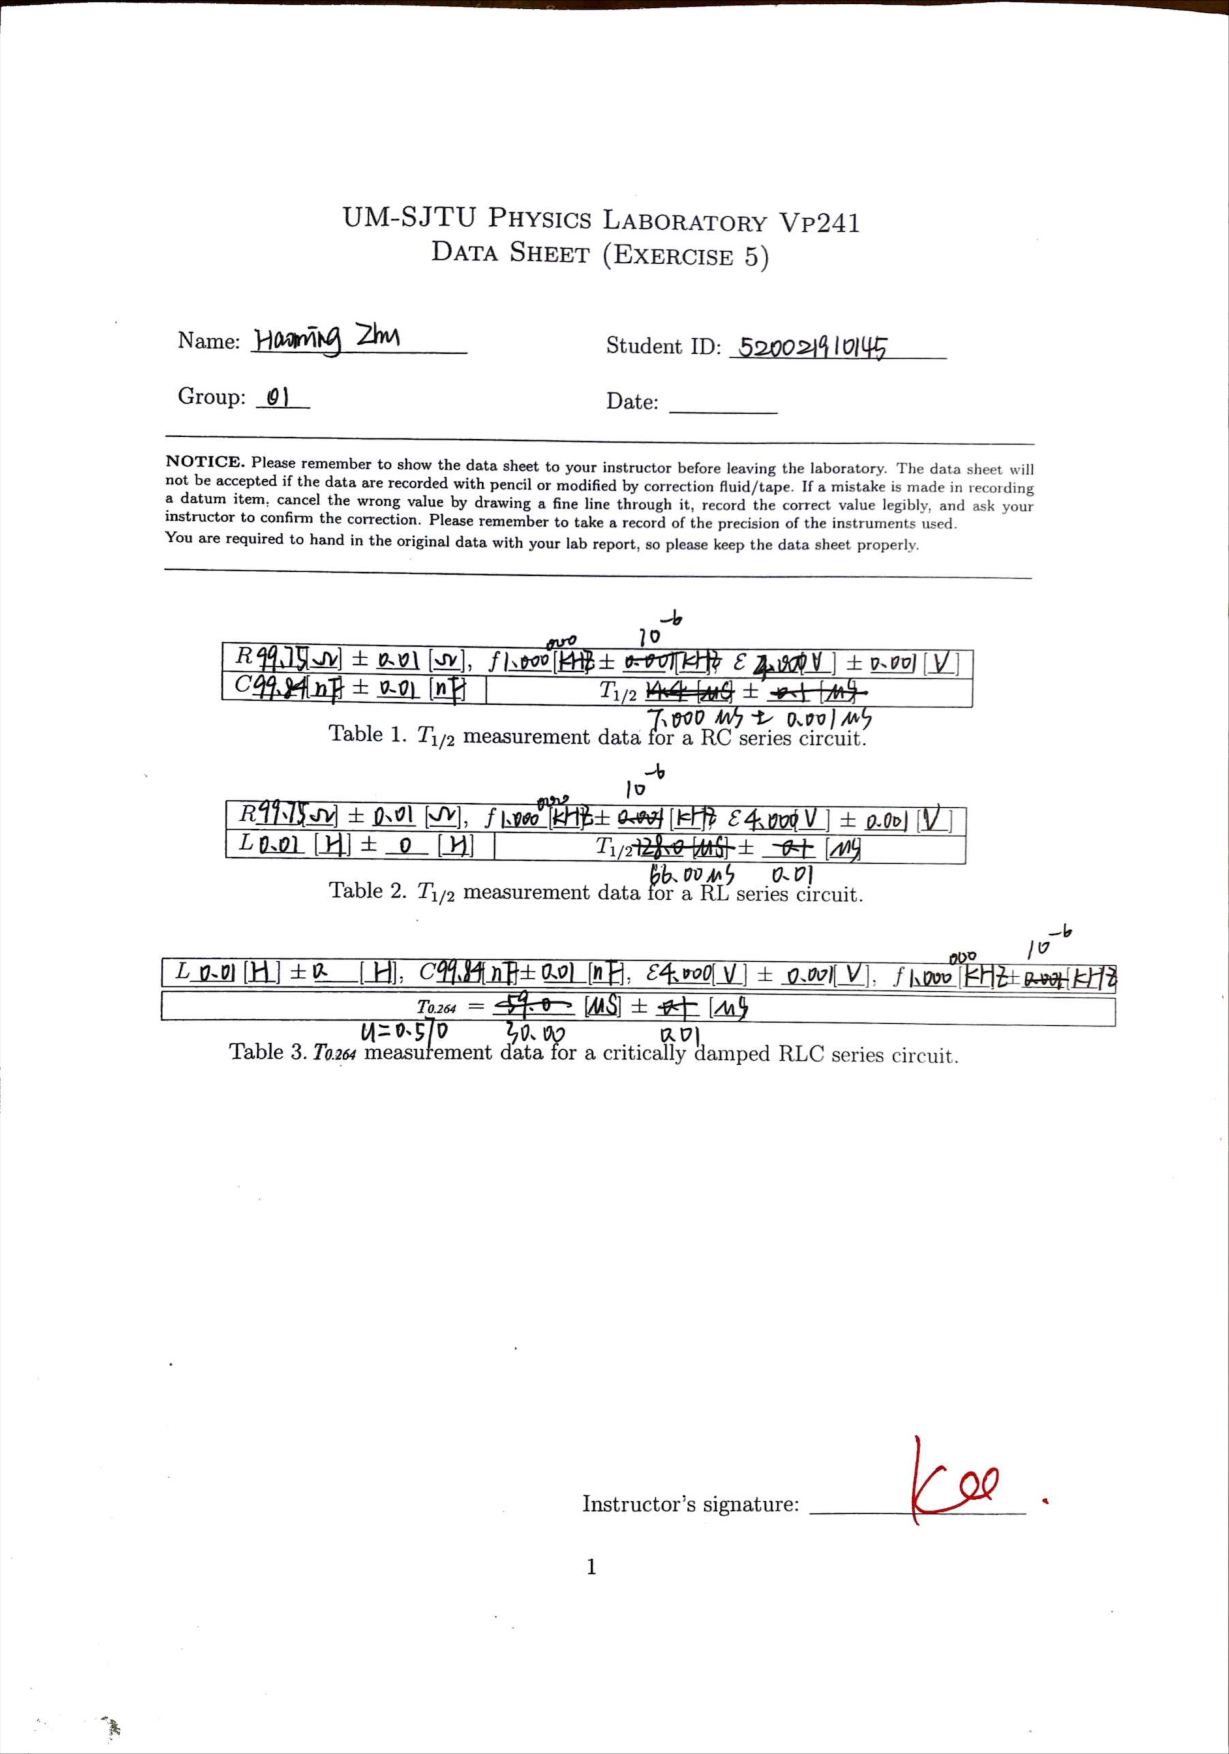
\includepdf[pages=-]{lab5_datasheet.pdf}

\end{document}	